\date{}
\title{}
\date{}
\begin{document}
\begin{frame}
    \titlepage
\end{frame}


\makeatletter
\newenvironment<>{btHighlight}[1][]
{\begin{onlyenv}#2\begingroup\tikzset{bt@Highlight@par/.style={#1}}\begin{lrbox}{\@tempboxa}}
{\end{lrbox}\bt@HL@box[bt@Highlight@par]{\@tempboxa}\endgroup\end{onlyenv}}

\newcommand<>\btHL[1][]{%
  \only#2{\begin{btHighlight}[#1]\bgroup\aftergroup\bt@HL@endenv}%
}
\def\bt@HL@endenv{%
  \end{btHighlight}%   
  \egroup %
}
\tikzset{
    btHLbox/.style={
        fill=red!30,outer sep=0pt,inner xsep=1pt, inner ysep=0pt, rounded corners=3pt
    },
}
\newcommand{\bt@HL@box}[2][]{%
  \tikz[#1]{%
    \pgfpathrectangle{\pgfpoint{1pt}{0pt}}{\pgfpoint{\wd #2}{\ht #2}}%
    \pgfusepath{use as bounding box}%
    \node[text width={},draw=none,anchor=base west, btHLbox, minimum height=\ht\strutbox+1pt,#1]{\raisebox{1pt}{\strut}\strut\usebox{#2}};
  }%
}

\lst@CCPutMacro
    \lst@ProcessOther {"2A}{%
      \lst@ttfamily 
         {\raisebox{2pt}{*}}% used with ttfamily
         {\raisebox{2pt}{*}}}% used with other fonts
    \@empty\z@\@empty

\lstdefinelanguage
   [x8664gas]{Assembler}     % add a "x64" dialect of Assembler
   [x86masm]{Assembler} % based on the "x86masm" dialect
   % with these extra keywords:
   {morekeywords={CDQE,CQO,CMPSQ,CMPXCHG16B,JRCXZ,LODSQ,MOVSXD,%
                  POPFQ,PUSHFQ,SCASQ,STOSQ,IRETQ,RDTSCP,SWAPGS,.TEXT,.STRING,.ASCIZ,%
                  BEQ,LW,SW,LB,SB,ADDIU,J,BEQZ,BNEZ,BNE,%
                  MOVUPD,MULPD,MOVSD,MULSD,%
                  SHLADD,MOV,CMP.LT,TBIT.NZ,BR.RET.SPTK.MANY,%
                  ADDQ,POPQ,PUSHQ,RRMOVQ,MRMOVQ,RMMOVQ,IRMOVQ,%
                  <-,LL,SC,ADDI,ADDL,VMOVDQA,ADDQ,CMPL,JB,JBE,MOVL,CLTQ,%
                  MOVW,PUSHW,MOV,ADD,SUB,INT,PUSH,MOV,ADD,REP,MOVSB,%
                  TESTQ,CMPQ,MOVL,MOVQ,ADDQ,JMPQ,XORQ,%
                  LEAQ,LEAL,LEA,RETQ,RET,POPL,POPW,PUSHL,PUSHW,%
                  LEAW,%
                  SUBQ,SYSCALL,.ASCII,CALLQ,MOVSLQ,JMP,ANDQ,SHRQ,MOVB,INCQ,TESTL,XORL,%
                  SHRL,LEAL,SARL,SUBL,IMULL,IMULQ,MOVDQU,PADDD,XORL,%
                  MOVZBL,MOVZB,SHRB,SRAL,SHRL,ANDL,%
                  CMOVNS,SRAL,SRAQ,MOVZBW,MOVZBQ,%
                  PADDW,PADDQ,MODUPS,MOVAPD,%
                  MOVL,RET,.GLOBL,%
		  PAUSE,LFENCE,JMP,%
                  },
    deletekeywords={eax,ebx,sp,si,cx,di,ds,cs,es,fs,dx,ax,bx,al,esi,ebp,ecx,rip,eip,edx,edi,rdi,esp},
    deletekeywords=[2]{size},
    alsoletter={\%},
    alsoother={()},
    emphstyle={\color{violet!50!black}},
    emph={\%rax,\%rbx,\%rcx,\%rdx,\%r8,\%r9,\%r10,\%r11,\%r12,\%r13,\%r14,\%r15,\%eax,\%ebx,\%sp,\%si,\%cx,\%di,\%ds,\%cs,\%es,\%fs,\%dx,\%ax,\%bx,\%al,\%esi,\%ebp,\%ecx,\%rip,\%eip,\%edx,\%edi,\%rdi,\%esp,\%rsp},
    %moreemph={eax,ebx,sp,si,cx,di,ds,cs,es,fs,dx,ax,bx,al,esi,ebp,ecx,rip,eip,edx,edi,rdi,esp},
    morecomment=[l]{\#},
    morecomment=[l]{\/\/},
    morecomment=[s]{/*}{*/},
    sensitive=false,
    keepspaces=true} % et

\lstalias[]{myasm}[x8664gas]{Assembler}

\lstdefinelanguage{JavaScript}{
  keywords={typeof, new, true, false, catch, function, return, null, catch, switch, var, if, in, while, do, else, case, break},
  ndkeywords={class, export, boolean, throw, implements, import, this},
  sensitive=false,
  comment=[l]{//},
  morecomment=[s]{/*}{*/},
  morestring=[b]',
  morestring=[b]"
}

\newcommand{\keywordstyle}{\sourcecodeprolight\bfseries\color{blue!30!black}}
\newcommand{\stringstyle}{\color{blue!20!black}\ttfamily}

\lstset{
    language=C,
    basicstyle=\sourcecodepro\EmptyMapping,
    escapechar=`,
    keywordstyle=\keywordstyle\EmptyMapping,
    identifierstyle=\sourcecodepro\EmptyMapping,
    numberstyle=\small\color{black!70},
    commentstyle=\color{red!60!black}\ttfamily\itshape,
    stringstyle=\color{blue!20!black}\ttfamily,
    ndkeywordstyle=\bfseries\color{blue!30!black},
    upquote=true,
}



\lstdefinestyle{medium}{
    basicstyle=\sourcecodepro\EmptyMapping\fontsize{12}{13}\selectfont,
    keywordstyle=\sourcecodepro\EmptyMapping\fontsize{12}{13}\selectfont\keywordstyle,
}

\lstdefinestyle{small}{
    basicstyle=\sourcecodepro\EmptyMapping\small,
    keywordstyle=\sourcecodepro\EmptyMapping\small\keywordstyle,
}

\lstdefinestyle{smaller}{
    basicstyle=\sourcecodepro\EmptyMapping\fontsize{11}{12}\selectfont,
    keywordstyle=\sourcecodepro\EmptyMapping\fontsize{11}{12}\selectfont\keywordstyle,
}

\lstdefinestyle{size105}{
    basicstyle=\sourcecodepro\EmptyMapping\fontsize{10.5}{11.5}\selectfont,
    keywordstyle=\sourcecodepro\EmptyMapping\fontsize{10.5}{11.5}\selectfont\keywordstyle,
}

\lstdefinestyle{size10}{
    basicstyle=\sourcecodepro\EmptyMapping\fontsize{10}{11}\selectfont,
    keywordstyle=\sourcecodepro\EmptyMapping\fontsize{10}{11}\selectfont\keywordstyle,
}


\lstdefinestyle{script}{
    basicstyle=\sourcecodepro\EmptyMapping\scriptsize,
    keywordstyle=\sourcecodepro\EmptyMapping\scriptsize\bfseries,
}




\begin{frame}
\frametitle{last time}
    \begin{itemize}
        \item DNS hierarchy
            \begin{itemize}
            \item labels starting at end
            \item zones with sets of authoritative servers
            \item zones might not match one to one with labels
                \begin{itemize}
                \item example virginia.edu/its.virginia in same zone, but cs.virginia.edu separate
                \end{itemize}
            \end{itemize}
        \item recursive versus authoritative servers
        \item caching and time-to-live
        \item smooth DNS handovers
        \item DNS record types, wire format
    \end{itemize}
\end{frame}

\begin{frame}
\frametitle{note on quiz Q4}
    \begin{itemize}
        \item \textit{customer P} had preference that one link was backup
        \item we asked about provider \textbf{Q's} announcements
            \begin{itemize}
                \item customer P can implement preference use local pref \\
                    (which takes precednece over everything but more specific usually)
            \end{itemize}
        \item these generally won't reflect P's preferences
            \vspace{.5cm}
        \item (Q gets paid regardless of which link P uses\ldots)
    \end{itemize}
\end{frame}


\section{primary, secondary, zone xfers}
\begin{frame}{primary and secondary servers}
\begin{itemize}
\item usually have multiple DNS servers for each zone
    \begin{itemize}
    \item needed to handle outages
    \end{itemize}
\item DNS protocol supports \textit{zone transfers} to synchronize them
    \begin{itemize}
    \item DNS query for type \texttt{AXFR} returns all RRs as special case
    \item (most public DNS servers block this from `normal'users)
    \end{itemize}
\item one server designed as `primary'; others are `secondary'
\item special SOA (start of authority) record provides metadata about zone
    \begin{itemize}
    \item name of primary server to contact
    \item serial number for current version (to quickly check if update)
    \item how long to wait between updates, etc.
    \end{itemize}
\end{itemize}
\end{frame}
 % FIXME: more detail?

\section{DNS query+answer format}
\begin{frame}{DNS messages (1)}
    \begin{itemize}
    \item client sends query to server
    \item server responds with response
    \vspace{.5cm}
    \item response and query have same format
        \begin{itemize}
        \item but different fields set/used
        \end{itemize}
    \end{itemize}
\end{frame}

\begin{frame}{DNS header}
\begin{tikzpicture}
\tikzset{
    blabel/.style={font=\small},
    blabel alt/.style={font=\fontsize{9}{10}\selectfont},
    flag/.style={alt=<2>{fill=red!10}},
    opcode/.style={alt=<3>{fill=red!10}},
    rcode/.style={alt=<4>{fill=red!10}},
}
\begin{scope}[yshift=0cm,x=0.45cm]
    \draw (0, 0) rectangle ++(16, -1) node[midway,blabel] {ID};
    \draw[flag] (16, 0) rectangle ++(1, -1) node[midway,blabel alt] {QR};
    \draw[opcode] (17, 0) rectangle ++(4, -1) node[midway,blabel] {opcode};
    \draw[flag] (21, 0) rectangle ++(1, -1) node[midway,blabel alt] {AA};
    \draw[flag] (22, 0) rectangle ++(1, -1) node[midway,blabel alt] {TC};
    \draw[flag] (23, 0) rectangle ++(1, -1) node[midway,blabel alt] {RD};
    \draw[flag] (24, 0) rectangle ++(1, -1) node[midway,blabel alt] {RA};
    \draw (25, 0) rectangle ++(1, -1) node[midway,blabel] {\tt 0};
    \draw[flag] (26, 0) rectangle ++(1, -1) node[midway,blabel alt] {AD};
    \draw[flag] (27, 0) rectangle ++(1, -1) node[midway,blabel alt] {CD};
    \draw[rcode] (28, 0) rectangle ++(4, -1) node[midway,blabel] {RCODE};
    \draw (0, -1) rectangle ++(16, -1) node[midway,blabel] {QDCOUNT (0 or 1)};
    \draw (16, -1) rectangle ++(16, -1) node[midway,blabel] {ANCOUNT};
    \draw (0, -2) rectangle ++(16, -1) node[midway,blabel] {NSCOUNT};
    \draw (16, -2) rectangle ++(16, -1) node[midway,blabel] {ARCOUNT};
    \draw (0, -3) rectangle ++(32, -1.5) node[midway,blabel] {QDCOUNT questions};
    \draw (0, -4.5) rectangle ++(32, -1.5) node[midway,blabel] {
            ANCOUNT+NSCOUNT+ARCOUNT RRs
    };
    \coordinate (mark low) at (16, -2.1);
\end{scope}
\tikzset{
    explain box low/.style={at={(mark low)},draw=red,very thick,align=left,anchor=north,fill=white},
    explain box low2/.style={at={([yshift=-2cm]mark low)},
        font=\small,draw=red,very thick,align=left,anchor=north,fill=white},
}
    \begin{visibleenv}<2>
    \node[explain box low2] {
        `flags' \\
        QR = 1 if query, 0 if response \\
        AA = 1 if authoritative \\
        TC = 1 if truncated (packet size limit) \\
        RD = 1 if query wants recursion (contact other servers) \\
        RA = 1 if server supports recursion  \\
        ~ \\
        DNSSEC (PKI for DNS) additions: \\
        AD = 1 if verified cryptographically (`authentic data') \\
        CD = 1 if no cryptographic check requested (`checking disabled') \\
    };
    \end{visibleenv}
    \begin{visibleenv}<3>
    \node[explain box low] {
        opcode \\
        0 for query \\
        some other operations
    };
    \end{visibleenv}
    \begin{visibleenv}<4>
    \node[explain box low] {
        response code, 0 for no error
    };
    \end{visibleenv}
\end{tikzpicture}
\end{frame}

\begin{frame}{caching `domain name does not exist'}
    \begin{itemize}
    \item when domain does not exist (RCODE=3, ``NXDOMAIN''):
    \vspace{.5cm}
    \item (RFC 2308)
    \item response should include SOA record
        \begin{itemize}
        \item recall: indicates primary server for zone and how often secondaries should update
        \end{itemize}
    \item can cache NXDOMAIN based on minimum of TTL and SOA record's update frequency
    \end{itemize}
\end{frame}

\begin{frame}{DNS message}
    \begin{itemize}
    \item header
    \item 0 or 1 question
        \begin{itemize}
        \item domain name + class + type
        \item (RR without TTL or value)
        \item special type values for ANY, some other things
        \end{itemize}
    \item ANCOUNT RRs in `answer section':
        \begin{itemize}
        \item CNAMEs (even if that's not the question type)
        \item matches for domain name (or CNAME) + class + type 
        \end{itemize}
    \item NSCOUNT+ARCOUNT RRs in `authority section' and `additional section
        \begin{itemize}
        \item not always included; usually NS or SOA records plus corresponding A/AAAA recods
        \end{itemize}
    \end{itemize}
\end{frame}


\section{DNS over UDP, TCP}
% size limitations
\begin{frame}{DNS over \ldots}
    \begin{itemize}
    \item UDP port 53
        \begin{itemize}
        \item send DNS message
        \item reply with DNS message back
        \end{itemize}
    \item TCP port 53
        \begin{itemize}
        \item send length (2B, big endian) + message
        \item reply with length (2B, big endian) + message
        \item (+ repeat)
        \end{itemize}
    \item over HTTPS (RFC 8484)
        \begin{itemize}
        \item using \url{https://server/dns-query}
        \end{itemize}
    \end{itemize}
\end{frame}

\begin{frame}[fragile]{DNS UDP size limit}
\begin{Verbatim}[fontsize=\fontsize{9}{10}]
$ dig virginia.edu txt +notcp +all
;; Truncated, retrying in TCP mode.

; <<>> DiG 9.18.28-0ubuntu0.22.04.1-Ubuntu <<>> virginia.edu txt +notcp +all
;; global options: +cmd
;; Got answer:
;; ->>HEADER<<- opcode: QUERY, status: NOERROR, id: 53043
;; flags: qr rd ra; QUERY: 1, ANSWER: 17, AUTHORITY: 0, ADDITIONAL: 1

;; OPT PSEUDOSECTION:
; EDNS: version: 0, flags:; udp: 65494
;; QUESTION SECTION:
;virginia.edu.			IN	TXT

;; ANSWER SECTION:
virginia.edu.		3537	IN	TXT	"cisco-ci-domain-verification=268b991de3589451b38fcfeaa99473f8e4fb2522f96a1b478e04ec1bd5a25ff9"
....
\end{Verbatim}
\end{frame}

\begin{frame}{DNS UDP size limit}
    \begin{itemize}
    \item 512 byte size limit for UDP
        \begin{itemize}
        \item if exceeded, set TC (truncate) flag and truncate response
        \item clients supposed to retry with TCP
        \end{itemize}
    \item extensions to DNS increase limit
        \begin{itemize}
        \item (but have to be opted into by clients)
        \end{itemize}
    \item explains why only 13 root server names
        \begin{itemize}
        \item 13 NS RRs + 13 A RRs $\approx$ 480 bytes (w/ name compression)
        \end{itemize}
    \end{itemize}
\end{frame}



\begin{frame}
\frametitle{sockets interlude}
    \begin{itemize}
    \item going to talk about sockets API for UDP/TCP
    \item then get back to some bonus DNS topics
    \end{itemize}
\end{frame}

\section{port numbers}
\begin{frame}{port numbers}
    \begin{itemize}
    \item we run multiple programs on a machine
        \begin{itemize}
        \item IP addresses identifying machine --- not enough
        \end{itemize}
    \item<2-> so, add 16-bit \textit{port numbers}
        \begin{itemize}
        \item<2-> think: multiple PO boxes at address
        \end{itemize}
    \vspace{.5cm}
    \item<3-> 0--49151: typically assigned for particular services
        \begin{itemize}
        \item 80 = http, 443 = https, 22 = ssh, \ldots
        \item usually <1024 reserved for sysadmin-only-use
        \end{itemize}
    \item<3-> 49152--65535: allocated on demand
        \begin{itemize}
        \item default ``return address'' for client connecting to server
        \end{itemize}
    \end{itemize}
\end{frame}

\begin{frame}{sockets}
    \begin{itemize}
    \item port number helps identify \textit{sockets}
    \item sockets = file applications use to access networks
    \end{itemize}
\end{frame}

\begin{frame}{port number independence}
    \begin{itemize}
    \item typically ``5-tuple'' identifies ``socket'': \\
        (protocol=TCP or UDP, source IP, dest IP, source port, dest port)
    \item means can have:
        \begin{itemize}
        \item two sockets with same source IP+source port, but different destinations
        \item two sockets with same dest IP+des port, but different sources
        \item two sockets with different protocols, but everything else same
        \end{itemize}
    \item special cases:
        \begin{itemize}
        \item dest IP/port can be `wildcard' (all zeroes usually)
        \item used for server that can be connected to
        \item used for unconnected UDP sockets
        \end{itemize}
    \end{itemize}
\end{frame}


\section{UDP}
\usetikzlibrary{patterns.meta}
\begin{frame}[fragile]{UDP format}
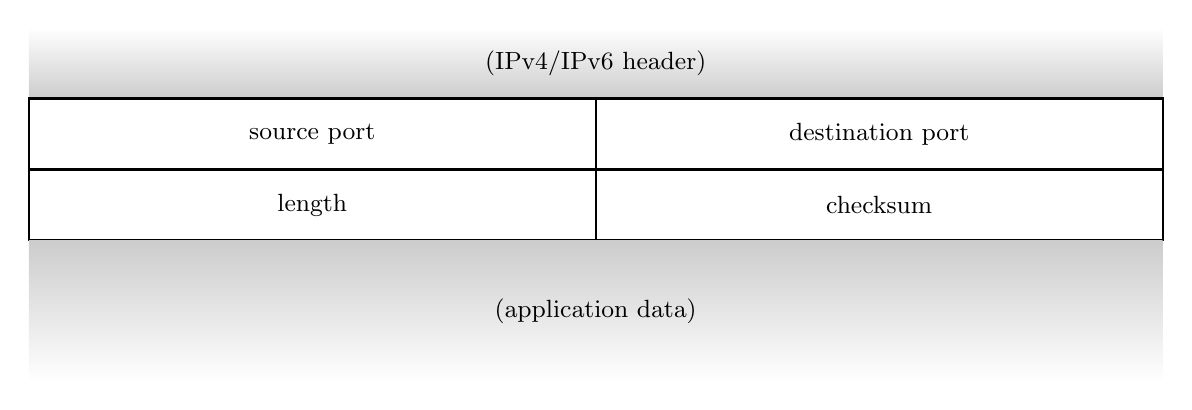
\begin{tikzpicture}
\tikzset{
    box/.style={draw,thick},
    label/.style={font=\small},
    label large/.style={},
    box label/.style={midway,font=\small,align=center},
    box label flags/.style={midway,font=\fontsize{8}{9}\selectfont,align=center},
    missing/.style={pattern=north west lines},
}
\begin{scope}[x=0.45cm,y=0.9cm]
\path[shading=axis,top color=white,bottom color=black!20] (0, 1) rectangle (32, 0)
    node[box label] {(IPv4/IPv6 header)};
\draw[box] (0, 0) rectangle (16, -1)
    node[midway,label] {source port};
\draw[box] (16, 0) rectangle (32, -1)
    node[midway,label] {destination port };
\draw[box] (0, -1) rectangle (16, -2)
    node[midway,label] {length};
\draw[box] (16, -1) rectangle (32, -2)
    node[midway,label] {checksum};
\path[shading=axis,bottom color=white,top color=black!20] (0, -2) rectangle (32, -4)
    node[box label] {(application data)};
\end{scope}
\end{tikzpicture}
\end{frame}


\section{BSD socket history}
\begin{frame}{BSD sockets}
    \begin{itemize}
    \item BSD = Berkely Standard Distribution (of Unix)
    \item interface designed for stream connections
    \item current C version standardized by POSIX
    \item pretty much default interface programming with TCP connections
        \begin{itemize}
        \item \ldots across all platforms
        \end{itemize}
    \end{itemize}
\end{frame}


\section{UDP sockets}
\begin{frame}[fragile]{unconnected UDP sockets (Python)}
\begin{Verbatim}[fontsize=\small]
import socket
# ipv4
sock = socket.socket(socket.AF_INET, socket.SOCK_DGRAM)
sock = socket.socket(socket.AF_INET, socket.SOCK_DGRAM,
                     socket.IPPROTO_UDP)
# ipv6
sock = socket.socket(socket.AF_INET6, socket.SOCK_DGRAM)
sock = socket.socket(socket.AF_INET6, socket.SOCK_DGRAM,
                     socket.IPPROTO_UDP)

sock.bind((local_host, local_port))
# local_host == "0.0.0.0" (v4) or "::" (v6) for "all possible"

data1, (host1, port1) = sock.recvfrom(MAX_SIZE)
sock.sendto(data, (host2, port2))
\end{Verbatim}
\end{frame}

\begin{frame}[fragile]{unconnected UDP sockets (Python, generic)}
\begin{Verbatim}[fontsize=\fontsize{9}{10}\selectfont]
import socket
possible_local_addrs = socket.getaddrinfo(
        local_host, local_port,
        family=socket.AF_UNSPEC,
        type=socket.SOCK_DGRAM,
        flags=socket.AI_PASSIVE)

for af, socktype, proto, canonname, sockaddr in possible_local_addrs:
    sock = socket.socket(af, socktype, proto)
    sock.bind(sockaddr)
    # then use sock for recvfrom/sendto somehow
\end{Verbatim}
\end{frame}

\begin{frame}[fragile]{unconnected UDP sockets (Python, generic)}
\begin{Verbatim}[fontsize=\fontsize{9}{10}\selectfont]
import socket
possible_remote_addrs = socket.getaddrinfo(
        remote_host, remote_port,
        family=socket.AF_UNSPEC,
        type=socket.SOCK_DGRAM,
        flags=0)

for af, socktype, proto, canonname, sockaddr in possible_remote_addrs:
    sock = socket.socket(af, socktype, proto)
    try:
        # hope local_host is acceptable for 'af'?
        # maybe choose local_host based on 'af' value?
        sock.bind((local_host, local_addr))
        sock.sendto(data, ...)
        ...
    except ...:
        ...
        # hope another address works?
        continue
\end{Verbatim}
\end{frame}

\begin{frame}{aside: getaddrinfo}
    \begin{itemize}
    \item lookup host+port by name
    \item can handle both IPv4 and IPv6
    \item AI\_PASSIVE = for bind()
    \item returns list of addresses
        \begin{itemize}
        \item sometimes: just choose one address (send message to server)
        \item sometimes: want to make socket for each address (run server)
        \end{itemize}
    \end{itemize}
\end{frame}

\begin{frame}[fragile]{unconnected UDP sockets (C, IPv4)}
\begin{Verbatim}[fontsize=\fontsize{9}{10}\selectfont]
int fd = socket(AF_INET, SOCK_DGRAM, 0 /* or IPPROTO_UDP */);
/* for 10.1.2.3 port 12345 
   there are utility functions to help with this, so you 
   shouldn't actually construct local_addr manually like this */
struct sockaddr_in local_addr;
memset(&local_addr, 0, sizeof(local_addr);
local_addr.sin_family = AF_INET;
local_addr.sin_port = htons(12345);
local_addr.sin_addr.s_addr = htonl((10<<24)|(1<<16)|(2<<8)|3),
bind(fd, &local_addr, sizeof(local_addr));
struct sockaddr_in remote1, remote2;
recvfrom(fd, buffer1, buffer1_size, 0, &remote1, sizeof(remote1));
recvfrom(fd, buffer2, buffer2_size, 0, &remote2, sizeof(remote2));
struct sockaddr_in remote3 = ...;
sendto(fd, buffer3, buffer3_size, 0, &remote3, sizeof(remote3));
\end{Verbatim}
\end{frame}

\begin{frame}[fragile]{connected UDP sockets (Python)}
\begin{Verbatim}[fontsize=\small]
import socket
# ipv4
sock = socket.socket(socket.AF_INET, socket.SOCK_DGRAM)
# ipv6
sock = socket.socket(socket.AF_INET6, socket.SOCK_DGRAM)

sock.bind((local_host, local_port))
sock.connect((remote_host, remote_port))
sock.send(b"one datagram")
sock.send(b"another datagram")
remote_data1 = sock.recv(MAX_SIZE)
remote_data2 = sock.recv(MAX_SIZE)
\end{Verbatim}
\end{frame}

\begin{frame}{choosing v4/v6?}
    \begin{itemize}
    \item nicer to write applications that handle both
    \item \ldots without explicitly doing this differently
    \vspace{.5cm}
    \item later socket API for that is getaddrinfo()
        \begin{itemize}
        \item also exists in C, but lots of extra stuff to handle types, etc.
        \end{itemize}
    \end{itemize}
\end{frame}


% FIXME: rearrange to put UDP sockets first, then talk about TCP

\subsection{netstat (UDP)}
\begin{frame}[fragile]{netstat}
\begin{Verbatim}[fontsize=\fontsize{9}{10}]
$ netstat --udp -na
Active Internet connections (servers and established)
Proto Recv-Q Send-Q Local Address           Foreign Address         State      
udp        0      0 128.143.71.27:60001     0.0.0.0:*                          
udp        0      0 128.143.71.27:60002     0.0.0.0:*                          
udp        0      0 128.143.71.27:60003     0.0.0.0:*                          
...
udp        0      0 128.143.71.27:68        128.143.67.64:67        ESTABLISHED
...
udp        0      0 127.0.0.1:123           0.0.0.0:*                          
udp        0      0 0.0.0.0:38269           0.0.0.0:*                          
udp        0      0 0.0.0.0:55407           0.0.0.0:*                          
udp        0      0 0.0.0.0:55786           0.0.0.0:*                          
...
udp6       0      0 :::45631                :::*                               
udp6       0      0 :::111                  :::*                               
udp6       0      0 fe80::1a66:daff:fe2:123 :::*                               
...
\end{Verbatim}
\end{frame}


\section{TCP client sockets}
\begin{frame}[fragile,label=connSetupClientAddrInfo]{connection setup: client, TCP+IPv4}
\begin{lstlisting}[
    language=Python,style=smaller,
    moredelim={**[is][\btHL<2|handout:2>]{@2}{2@}},
    moredelim={**[is][\btHL<3|handout:3>]{@3}{3@}},
    moredelim={**[is][\btHL<4|handout:4>]{@4}{4@}},
    moredelim={**[is][\btHL<5|handout:5>]{@5}{5@}},
    moredelim={**[is][\btHL<6|handout:6>]{@6}{6@}},
]
sock = socket.socket(socket.AF_INET, socket.SOCK_STREAM)
# to select local host/port: socket.bind(('128.143.71.27', 54444))
# if no local host/port selected, OS assigns
sock.connect(('128.143.67.8', 443))
...
sock.send(...)
sock.recv(...)
\end{lstlisting}
\end{frame}

\begin{frame}[fragile,label=connSetupClientAddrInfo]{connection setup: client, TCP+IPv6}
\begin{lstlisting}[
    language=Python,style=smaller,
    moredelim={**[is][\btHL<2|handout:2>]{@2}{2@}},
    moredelim={**[is][\btHL<3|handout:3>]{@3}{3@}},
    moredelim={**[is][\btHL<4|handout:4>]{@4}{4@}},
    moredelim={**[is][\btHL<5|handout:5>]{@5}{5@}},
    moredelim={**[is][\btHL<6|handout:6>]{@6}{6@}},
]
sock = socket.socket(socket.AF_INET6, socket.SOCK_STREAM)
# to select local host/port: socket.bind(('3fff:1234::1', 54444))
# if no local host/port selected, OS assigns
sock.connect(('2607:f8b0:4004:c06::67', 443))
...
sock.send(...)
sock.recv(...)
\end{lstlisting}
\end{frame}


\begin{frame}[fragile,label=connSetupClientAddrInfo]{connection setup: generic TCP, addrinfo}
\begin{Verbatim}[fontsize=\fontsize{9}{10}]
import socket
possible_addrs = socket.getaddrinfo(
        'www.cs.virginia.edu', '443',
        socket.AF_UNSPEC, socket.SOCK_STREAM)

for af, socktype, proto, canonname, sockaddr in possible_addrs:
    try:
        sock = socket.socket(af, socktype, proto)
    except OSError:
        sock = None
        continue
    try:
        sock.connect(sa)
    except OSError:
        sock.close()
        sock = None
        continue

if sock == None:
    # not successful
\end{Verbatim}
\end{frame}

 

\subsection{partial/split read/writes}
\usetikzlibrary{arrows.meta}
\begin{frame}{size mismatch? (1)}
\begin{tikzpicture}
\tikzset{>=Latex}
\node[anchor=south] at (1.5, 0) {one end};
\draw[ultra thick] (0, 0) -- ++(3, 0);
\draw[ultra thick] (10, 0) -- ++(3, 0);
\node[anchor=south] at (11.5, 0) {other end};
\node[font=\small] at (7, -.25) {(get \texttt{fd}s/\texttt{sock}s:)};
\tikzset{
    function/.style={font=\fontsize{9}{10}\tt\selectfont,align=left},
}
\node[function,anchor=east] (write 1) at (4, -1) {
sock.send(b"12345")
};
\node[function,anchor=west] (read 1) at (7, -2) {
b"123" == sock.recv(3) \\
b"45" == sock.recv(2) 
};
\draw[thick,->] (write 1) -- (read 1);
\end{tikzpicture}
\end{frame}

\begin{frame}{size mismatch? (2)}
\begin{tikzpicture}
\tikzset{>=Latex}
\node[anchor=south] at (1.5, 0) {one end};
\draw[ultra thick] (0, 0) -- ++(3, 0);
\draw[ultra thick] (10, 0) -- ++(3, 0);
\node[anchor=south] at (11.5, 0) {other end};
\node[font=\small] at (7, -.25) {(get \texttt{fd}s/\texttt{sock}s:)};
\tikzset{
    function/.style={font=\fontsize{9}{10}\tt\selectfont,align=left},
}
\node[function,anchor=east] (write 1) at (4, -1) {
sock.send(b"12") \\
sock.send(b"345")
};
\node[function,anchor=west] (read 1) at (7, -2) {
b"12345" == sock.recv(5)
};
\draw[thick,->] (write 1) -- (read 1);
\end{tikzpicture}
\end{frame}

\begin{frame}{partial reads?}
\begin{tikzpicture}
\tikzset{>=Latex}
\node[anchor=south] at (1.5, 0) {one end};
\draw[ultra thick] (0, 0) -- ++(3, 0);
\draw[ultra thick] (10, 0) -- ++(3, 0);
\node[anchor=south] at (11.5, 0) {other end};
\node[font=\small] at (7, -.25) {(get \texttt{fd}s/\texttt{sock}s:)};
\tikzset{
    function/.style={font=\fontsize{9}{10}\tt\selectfont,align=left},
}
\node[function,anchor=east] (write 1) at (4, -1) {
sock.send(b"X" * 6000)
};
\node[function,anchor=west] (read 1) at (7, -2) {
\textit{\normalfont sometimes} b"X" * 6000 == sock.recv(6000) \\
\textit{\normalfont or sometimes} \\
b"X" * 1490 == sock.recv(6000) \\
b"X" * 2980 == sock.recv(4510) \\
b"X" * 1530 == sock.recv(1530) 
};
\draw[thick,->] (write 1) -- (read 1);
\end{tikzpicture}
\end{frame}

\begin{frame}{partial writes}
\begin{tikzpicture}
\tikzset{>=Latex}
\node[anchor=south] at (1.5, 0) {one end};
\draw[ultra thick] (0, 0) -- ++(3, 0);
\draw[ultra thick] (10, 0) -- ++(3, 0);
\node[anchor=south] at (11.5, 0) {other end};
\node[font=\small] at (7, -.25) {(get \texttt{fd}s/\texttt{sock}s:)};
\tikzset{
    function/.style={font=\fontsize{9}{10}\tt\selectfont,align=left},
}
\node[function,anchor=east] (write 1) at (4, -1) {
sock.setblocking(False) \\
sock.send(b"X" * 6000) == 1480
};
\node[function,anchor=west] (read 1) at (7, -2) {
b"X" * 1480 == sock.recv(6000) \\
(+ no more data)
};
\draw[thick,->] (write 1) -- (read 1);
\end{tikzpicture}
\end{frame}

\begin{frame}{partial reads/writes}
    \begin{itemize}
    \item read/recv can have read less than requested
        \begin{itemize}
        \item read of zero bytes = end of file
        \end{itemize}
    \item send/write can write less than requested\ldots \\
        but only on error or if non-blocking mode requested
    \end{itemize}
\end{frame}

\begin{frame}{incomplete writes}
\begin{itemize}
    \item \texttt{send} might write less than requested
        \begin{itemize}
        \item error after writing some data
        \item if blocking disabled
        \end{itemize}
    \item \texttt{recv} might read less than requested
        \begin{itemize}
        \item error after reading some data
        \item not enough data got there in time
        \end{itemize}
\end{itemize}
\end{frame}


\subsection{simultaneous read/write}
\begin{frame}{reading and writing at once}
    \begin{itemize}
    \item so far assumption: alternate between reading+writing
        \begin{itemize}
        \item sufficient for FTP assignment
        \item how many protocols work
        \end{itemize}
    \item ``half-duplex''
    \item don't have to use sockets this way, but tricky
        \vspace{.5cm}
    \item threads: one reading thread, one writing thread \textit{OR}
    \item event-loop: use \textit{non-blocking I/O} and select()/poll()/etc. functions
        \begin{itemize}
        \item non-blocking I/O setup with fcntl() function
        \item non-blocking write() fills up buffer as much as possible, then returns
        \item non-blocking read() returns what's in buffer, never waits for more
        \end{itemize}
    \end{itemize}
\end{frame}


\section{TCP server sockets}
\subsection{server socket idea}
\usetikzlibrary{arrows.meta,calc}


\begin{frame}{sockets and server sockets (C)}
% FIXME
\begin{tikzpicture}
    \tikzset{
        >=Latex,
        comp box/.style={draw, thick, align=center, minimum width=1.5cm,minimum height=1.5cm},
        explain box/.style={draw=red,very thick, align=left},
        msg/.style={font=\small},
        cmd/.style={font=\small},
    }
    \node[draw,circle,label={south:client}] (client) {socket};
    \node[draw,circle,align=center] (ssocket) at ([xshift=8.75cm,yshift=4cm]client.west) {server\\socket};
    \node[draw,circle,align=center,label={south:server},visible on=<4->] (server) at ([xshift=8.75cm]client.west) {socket};
    \draw[very thick,dotted,<-] (ssocket.east) -- ++(.5cm,0cm) node[right,font=\small\tt,align=left] {
        server: \\
        \myemph<2>{ss\_fd = socket(\ldots)} \\
        \myemph<3>{bind(ss\_fd, addr, \ldots)} \\
        \myemph<3>{listen(ss\_fd, \ldots)}
    };
    \draw[very thick,dotted,<-] (client.north) -- ++(0cm,2cm) node[above,xshift=1cm,font=\small\tt,align=left] {
        client: \\
        \myemph<2>{fd = socket(\ldots)}
    };
    \begin{visibleenv}<2>
        \node[explain box,anchor=north] at ([yshift=-.5cm]ssocket.south) {
            socket() function --- create socket fd
        };
    \end{visibleenv}
    \begin{visibleenv}<3>
        \node[explain box,anchor=north] at ([yshift=-.5cm]ssocket.south) {
            listen() --- turn socket into server socket \\
            still has a file descriptor, but \ldots \\
            can only \texttt{accept()} --- create normal socket
        };
    \end{visibleenv}
    \begin{visibleenv}<4->
    \draw[very thick,dotted,->] (client) -- (ssocket)
        node[font=\small,midway,sloped,above,align=left] {request connection \\
                                   client: \texttt{\myemph<4-5>{connect(fd, addr, \ldots)}}};
    \draw[very thick,dotted,->,out=-120,in=120] (ssocket) to (server);
    \node[anchor=west,align=left] at ([xshift=-.75cm]$(server)!0.5!(ssocket)$) {server: \\ \texttt{fd = \myemph<4-5>{accept(ss\_fd, \ldots)}}};
    \end{visibleenv}
    \begin{visibleenv}<5->
    \draw[<->,double,ultra thick] (client) -- (server) node[midway,fill=white,inner sep=0.1mm] {connection};
    \end{visibleenv}
\end{tikzpicture}
\end{frame}


\begin{frame}{sockets and server sockets (Python)}
% FIXME
\begin{tikzpicture}
    \tikzset{
        >=Latex,
        comp box/.style={draw, thick, align=center, minimum width=1.5cm,minimum height=1.5cm},
        explain box/.style={draw=red,very thick, align=left},
        msg/.style={font=\small},
        cmd/.style={font=\small},
    }
    \node[draw,circle,label={south:client}] (client) {socket};
    \node[draw,circle,align=center] (ssocket) at ([xshift=7.75cm,yshift=4cm]client.west) {server\\socket};
    \node[draw,circle,align=center,label={south:server},visible on=<4->] (server) at ([xshift=8.75cm]client.west) {socket};
    \draw[very thick,dotted,<-] (ssocket.east) -- ++(.5cm,0cm) node[right,font=\small\tt,align=left] {
        server: \\
        \myemph<2>{ssock = \textbackslash} \\
        \myemph<2>{\hspace{.25cm}socket.socket(\ldots)} \\
        \myemph<3>{ssock.bind(\ldots)} \\
        \myemph<3>{ssock.listen()}
    };
    \draw[very thick,dotted,<-] (client.north) -- ++(0cm,2cm) node[above,xshift=1cm,font=\small\tt,align=left] {
        client: \\
        \myemph<2>{sock = socket.socket(\ldots)}
    };
    \begin{visibleenv}<2>
        \node[explain box,anchor=north] at ([yshift=-.5cm]ssocket.south) {
            socket() function --- create socket fd
        };
    \end{visibleenv}
    \begin{visibleenv}<3>
        \node[explain box,anchor=north] at ([yshift=-.5cm]ssocket.south) {
            listen() --- turn socket into server socket \\
            still has a file descriptor, but \ldots \\
            can only \texttt{accept()} --- create normal socket
        };
    \end{visibleenv}
    \begin{visibleenv}<4->
    \draw[very thick,dotted,->] (client) -- (ssocket)
        node[font=\small,midway,sloped,above,align=left] {request connection \\
                                   client: \texttt{\myemph<4-5>{sock.connect(\ldots)}}};
    \draw[very thick,dotted,->,out=-120,in=120] (ssocket) to (server);
    \node[anchor=west,align=left] at ([xshift=-.75cm]$(server)!0.5!(ssocket)$) {server: \\ \texttt{sock, addr = \textbackslash} \\ \hspace{.25cm}\myemph<4-5>{\texttt{ssock.accept(\ldots)}}};
    \end{visibleenv}
    \begin{visibleenv}<5->
    \draw[<->,double,ultra thick] (client) -- (server) node[midway,fill=white,inner sep=0.1mm] {connection};
    \end{visibleenv}
\end{tikzpicture}
\end{frame}



\subsection{TCP server setup}
\begin{frame}[fragile]{connection setup: server, IPv4}
\begin{Verbatim}[fontsize=\small]
import socket
ssock = socket.socket(socket.AF_INET, socket.SOCK_STREAM)
# 0.0.0.0 == "any IP address"
ssock.bind(('0.0.0.0', 12345))
ssock.listen()
sock, remote_addr = ssock.accept()
Use(sock)
\end{Verbatim}
\end{frame}

\begin{frame}[fragile]{connection setup: server, IPv4}
\begin{Verbatim}[fontsize=\small]
import socket
ssock = socket.socket(socket.AF_INET, socket.SOCK_STREAM)
# 0.0.0.0 == "any IP address"
ssock.bind(('0.0.0.0', 12345))
ssock.listen()
sock, remote_addr = ssock.accept()
Use(sock)
\end{Verbatim}
\end{frame}

\begin{frame}[fragile,label=connSetupServerLookup]{connection setup: server, generic}
\begin{Verbatim}[fontsize=\fontsize{9}{10}]
import select
import socket
all_addrs = socket.getaddrinfo(
        None, '12345',
        socket.AF_UNSPEC, socket.SOCK_STREAM)
ssocks = []
for af, socktype, proto, canonname, sockaddr in possible_addrs:
    ssock = socket.socket(af, socktype, proto)
    try:
        ssock.bind(sockaddr)
        ssock.listen()
        ssocks.append(ssock)
    except OSError:
        pass

which_ready, _, _ = select.select(ssocks, [], [])
for item in which_ready:
    sock, remote_addr = which_ready.accept()
    Use(sock)
\end{Verbatim}
\end{frame}



\section{connection internals/socket tracking}
\subsection{TCP handshake}
\begin{frame}{three-way TCP handshake}
\begin{tabular}{l@{$\rightarrow$}l|llll}
from & to & flags & seq & ack & data\\
client & server & SYN & $X$ & --- & ---\\
server & client & SYN+ACK & $Y$ & $X+1$ & ---\\
client & server & ACK & $X+1$ & $Y+1$ & ---\\
client & server & ACK & $X+1$ & $Y+1$ & initial data  \\
\end{tabular}
$X$, $Y$ selected at random
\end{frame}

\begin{frame}
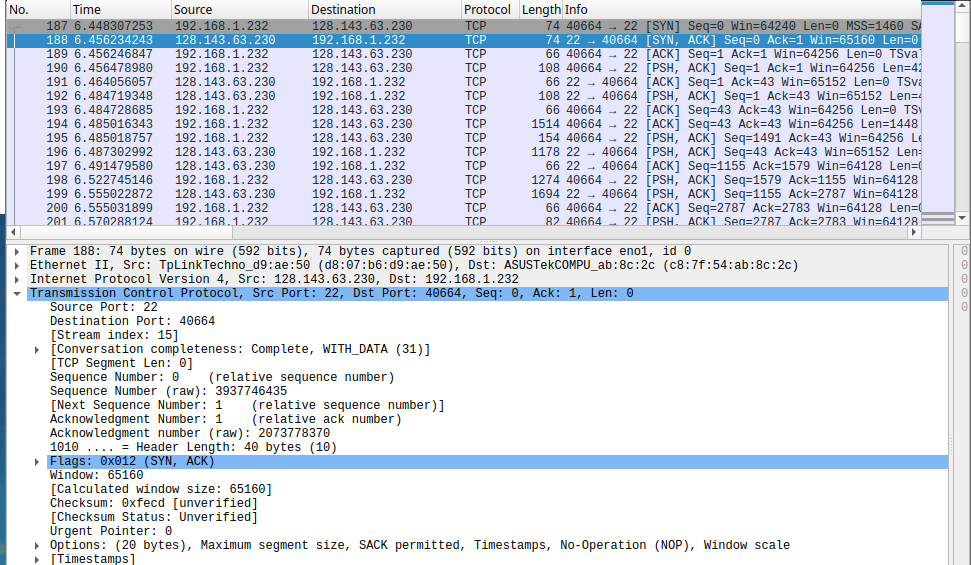
\includegraphics[width=\textwidth]{../sockets/tcp-handshake-wireshark}
\end{frame}

\begin{frame}[fragile]{so many messages?}
    \begin{itemize}
    \item TCP waits full round-trip before sending data; can do better
    \item example: QUIC (figure from RFC 9000, TCP+TLS replacement)
    \end{itemize}
\begin{Verbatim}[fontsize=\fontsize{8}{9}\selectfont]
Client                                                  Server

Initial[0]: CRYPTO[CH]
0-RTT[0]: STREAM[0, "..."] ->

                                 Initial[0]: CRYPTO[SH] ACK[0]
                                  Handshake[0] CRYPTO[EE, FIN]
                          <- 1-RTT[0]: STREAM[1, "..."] ACK[0]

Initial[1]: ACK[0]
Handshake[0]: CRYPTO[FIN], ACK[0]
1-RTT[1]: STREAM[0, "..."] ACK[0] ->

                                          Handshake[1]: ACK[0]
         <- 1-RTT[1]: HANDSHAKE_DONE, STREAM[3, "..."], ACK[1]

Figure 6: Example 0-RTT Handshake
\end{Verbatim}
\end{frame}


\subsection{TCP state machine}
\begin{frame}{TCP state machine}
\begin{tikzpicture}
\node (state) {
    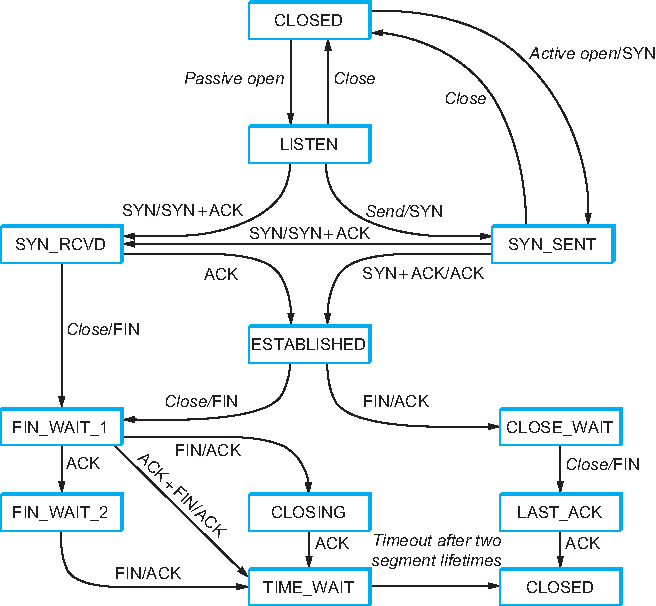
\includegraphics[height=0.8\textheight]{../sockets/sysapproach-tcp-state-fig}
};
\node[anchor=north west] at (state.north east) {
   notation: event/action  \\
   ~ \\
   not shown explicitly: timeout/resend
};
\end{tikzpicture}
\end{frame}


\begin{frame}{connection close}
    \begin{itemize}
    \item FIN (I want to close) + ACK (confirm close)
    \vspace{.5cm}
    \item ACK side needs to wait just in case FIN resent
        \begin{itemize}
        \item keep port number from being reused
        \item TIME\_WAIT state
        \end{itemize}
    \end{itemize}
\end{frame}

\begin{frame}{RST}
    \begin{itemize}
    \item RST (reset) flag often used to respond to unexpected packets
    \item example: data packet for never-established connection
    \end{itemize}
\end{frame}


\subsection{netstat (TCP)}

\begin{frame}[fragile,label=laptopNetstat]{connections on my desktop}
\begin{lstlisting}[language={},basicstyle=\fontsize{9.5}{10.5}\selectfont]
cr4bd@reiss-t3620
: /zf14/cr4bd ; netstat --inet --inet6 --numeric
Active Internet connections (w/o servers)
Proto Recv-Q Send-Q Local Address           Foreign Address         State      
tcp        0      0 128.143.67.91:49202     128.143.63.34:22        ESTABLISHED
tcp        0      0 128.143.67.91:803       128.143.67.236:2049     ESTABLISHED
tcp        0      0 128.143.67.91:50292     128.143.67.226:22       TIME_WAIT  
tcp        0      0 128.143.67.91:54722     128.143.67.236:2049     TIME_WAIT  
tcp        0      0 128.143.67.91:52002     128.143.67.236:111      TIME_WAIT  
tcp        0      0 128.143.67.91:732       128.143.67.236:63439    TIME_WAIT  
tcp        0      0 128.143.67.91:40664     128.143.67.236:2049     TIME_WAIT  
tcp        0      0 128.143.67.91:54098     128.143.67.236:111      TIME_WAIT  
tcp        0      0 128.143.67.91:49302     128.143.67.236:63439    TIME_WAIT  
tcp        0      0 128.143.67.91:50236     128.143.67.236:111      TIME_WAIT  
tcp        0      0 128.143.67.91:22        172.27.98.20:49566      ESTABLISHED
tcp        0      0 128.143.67.91:51000     128.143.67.236:111      TIME_WAIT  
tcp        0      0 127.0.0.1:50438         127.0.0.1:631           ESTABLISHED
tcp        0      0 127.0.0.1:631           127.0.0.1:50438         ESTABLISHED
\end{lstlisting}
\end{frame}
% FIXME: flow chart




\section{more socket customization}
\subsection{setsockopt}
\begin{frame}[fragile]{socket options}
\begin{itemize}
\item `socket options' for extra settings
\item Python: \texttt{sock.setsockopt(level, key, value)}
\item C: \texttt{setsockopt(sock, level, key, value)}
\vspace{.5cm}
\item common level values
    \begin{itemize}
    \item \texttt{SOL\_SOCKET} --- OS-level
    \item \texttt{IPPROTO\_IP}
    \item \texttt{IPPROTO\_IPV4}
    \item \texttt{IPPROTO\_TCP}
    \end{itemize}
\end{itemize}
\end{frame}

\begin{frame}{common SOL\_SOCKET options}
    \begin{itemize}
    \item \texttt{SO\_REUSEADDR} --- allow bind()ing even if another socket for this port active
        \begin{itemize}
        \item common problem: server can't bind() because old session in TIME\_WAIT
        \end{itemize}
    \item \texttt{SO\_RCVBUF} --- buffer size used by OS for receiving bytes
    \item \texttt{SO\_SNDBUF} --- buffer size used by OS for sending bytes
    \vspace{.5cm}
    \item (full list on Linux: \texttt{man 7 socket})
    \end{itemize}
\end{frame}



\subsection{Nagle, etc.}
\begin{frame}[fragile]{efficiency problem}
\begin{Verbatim}[fontsize=\small]
sock = ...
sock.send(b'About to send file with 16Kbytes')
sock.send(b'File is HTML; updated 16 November')
sock.send(file_data)
\end{Verbatim}
\begin{itemize}
\item Naive approach:
    \begin{itemize}
    \item one packet for `about to send file with\ldots'
    \item one packet for `file is HTML; \ldots'
    \item some number of packets for \texttt{file\_data}
    \end{itemize}
\item sending small TCP packets, so lots of overhead
\end{itemize}
\end{frame}

\begin{frame}{Nagle's algorithm}
\begin{itemize}
\item (RFC 896)
\item delay sending data when smaller than full TCP segment
\item hope: by waiting we'll get a full TCP segment
    \begin{itemize}
    \item typical wait: 200 ms?
    \end{itemize}
\vspace{.5cm}
\item TCP\_NODELAY socket option can disable (at least on Linux)
\end{itemize}
\end{frame}


\section{broadcast}
\begin{frame}{broadcast/multicast}
\begin{itemize}
\item IPv4: can broadcast to every machine on local network
    \begin{itemize}
    \item set the SO\_BROADCAST socket option to 1
    \item send to special address 255.255.255.255 
    \item received at that port number on all machines
    \end{itemize}
\item multicast (send-to-many) groups
    \begin{itemize}
    \item request to receive: IP\_ADD\_MEMBERSHIP (v4), IPV6\_ADD\_MEMBERSHIP (v6)
    \item each `multicast group' has IP address
    \item 224.0.0.0/24 and ff02::/16 = local network only
    \item local network version usually implemented by broadcasting + filtering by IP
    \item (non-local-network multicast is more complex\ldots)
    \end{itemize}
\end{itemize}
\end{frame}

\begin{frame}{service discovery}
\begin{itemize}
\item example: find printers on local network automatically
\vspace{.5cm}
\item typical protocol mDNS (`multicast DNS')
\item uses IP addressses 224.0.0.251 / ff02::fb + port 5353
\item all machines on local network receive from all other machines on local network
\end{itemize}
\end{frame}


\section{aside: other address families}
\begin{frame}{other address families}
    \begin{itemize}
    \item AF\_UNIX {\small (= AF\_LOCAL in C, but not Python)}
        \begin{itemize}
        \item sockets can be represented in files on disk
        \item support sending file descriptors usually
        \end{itemize}
    \item (not sure how portable?) AF\_RAW
        \begin{itemize}
        \item usually how wireshark captures packets on Linux
        \item also supports writing packets
        \end{itemize}
    \item (Linux only) AF\_NETLINK 
        \begin{itemize}
        \item communicate with kernel networking code
        \end{itemize}
    \item AF\_AX25, AF\_APPLETALK, AF\_DECNET, \ldots
        \begin{itemize}
        \item other interesting protocols
        \end{itemize}
    \end{itemize}
\end{frame}



\begin{frame}
\frametitle{end of sockets interlude}
    \begin{itemize}
        \item back to DNS
    \end{itemize}
\end{frame}



\section{DNS extensions, briefly}
% OPT pseudorecord; EDNS0; DNSSEC
\begin{frame}{eDNS(0) (RFC 6891)}
    \begin{itemize}
    \item extend DNS protocol by sending psuedo-RR
        \begin{itemize}
        \item added in additoinal section of requests
        \item name \texttt{.} (empty)
        \item type OPT/44
        \item CLASS, TTL fields reused for other stuff
        \end{itemize}
    \item specifies:
        \begin{itemize}
        \item \myemph{max size over UDP}
        \item extra bits for RCODE
        \item additoinal, variable length data
        \end{itemize}
    \end{itemize}
\end{frame}


\section{cache poisoning}
% spoofing protections
    % port numbers, IDs, capitalization, TCP

\usetikzlibrary{arrows.meta,calc,fit,matrix,shapes,shapes.misc}
\providecommand{\computer}{%
    
\includegraphics[width=1cm]{../common/Noun_project_216.pdf}
}
\providecommand{\computerAlt}{%
    
\includegraphics[width=1cm]{../common/Noun_project_alt_cpu.pdf}
}
\providecommand{\switch}{%
    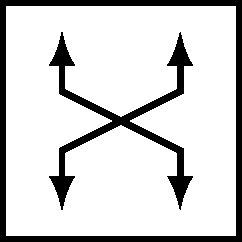
\includegraphics[width=0.9cm]{../common/fig-switch.pdf}
}
\providecommand{\router}{%
    
\includegraphics[width=0.9cm]{../common/fig-router.pdf}
}


\begin{frame}{DNS cache poisoning}
\begin{tikzpicture}
\tikzset{
    computer/.style={inner sep=0mm,outer sep=0mm,execute at begin node={\computer}},
    computer alt/.style={inner sep=0mm,outer sep=0mm,execute at begin node={\computerAlt}},
    connect/.style={draw,very thick,Latex-Latex},
    connect big/.style={draw,ultra thick,Latex-Latex},
    network/.style={cloud,draw,aspect=2},
    marked/.style={draw,line width=1mm,blue,dotted},
    marked pack/.style={draw,solid,line width=0.8mm,draw=blue,fill=white,align=left,
        font=\small},
    marked alt/.style={draw,line width=1mm,violet,dotted},
    marked pack alt/.style={draw,solid,line width=0.8mm,draw=violet,fill=white,align=left,
        font=\small},
};

\node[computer] (attacker) at (0, 2) {};
\node[computer] (attacker2) at (0, -4) {};
\node[font=\huge] at (attacker) {\emoji{smiling-face-with-horns}};
\node[font=\huge] at (attacker2) {\emoji{smiling-face-with-horns}};
\node[computer] (victim) at (0, -2) {};
\node[network] (net) at (3.5, 0) {~~};
\node[network] (net2) at (5, -4) {~~};
\node[computer,label={south:dns.isp.com}] (resolver) at (7, 2) {};
\node[computer,label={south:ns.foo.com}] (authority) at (10, -4) {};
%
\draw[connect] (attacker) -- (net);
\draw[connect] (victim) -- (net);
\draw[connect] (net) -- (net2);
\draw[connect] (net) -- (resolver);
\draw[connect] (net2) -- (authority);
\draw[connect] (net2) -- (attacker2);
%
\begin{visibleenv}<2>
\draw[marked,-Latex] (attacker) -- ([yshift=.1cm]net.center) 
    node[pos=0.25,above right,marked pack] {
        \emoji{smiling-face-with-horns} user $\rightarrow$ dns.isp.com: \\
        foo.com IN A ?
    } -- (resolver.west);
\end{visibleenv}
\begin{visibleenv}<3>
\draw[marked,-Latex] (resolver.south) -- ([yshift=-.1cm]net.center) 
    node[pos=0.25,above right,marked pack] {
        dns.isp.com $\rightarrow$ ns.foo.com: \\
        foo.com IN A ?
    } -- (net2.center) -- (authority);
\end{visibleenv}
\begin{visibleenv}<3>
\draw[marked,-Latex] (attacker2) -- (net2.center)
    node[pos=0.25,marked pack,above right] {
        ns.foo.com $\rightarrow$ dns.isp.com: \\
        foo.com 9999999 IN A (attcker's IP) 
    }
    -- ([yshift=-.2cm]net.center) -- ([yshift=-.2cm]resolver.west);
\node[anchor=north west,draw=red,ultra thick,align=left,font=\small] at ([xshift=2cm]resolver.north east) {
    attacker's `spoofed' response \\
    causes dns.isp.com to record \\
    wrong IP
};
\end{visibleenv}
\begin{visibleenv}<4>
\draw[marked,-Latex] (victim) -- (net) node[pos=0.25,above right,marked pack] {
       innocent user $\rightarrow$ dns.isp.com: \\
       foo.com IN A ?
}
    -- (resolver.west);

\draw[marked,-Latex] (resolver.south) -- (net) node[pos=0.25,above right,marked pack] {
       dns.isp.com $\rightarrow$  dns.isp.com: \\
       foo.com 9999944 IN A (attacker's IP)
    }
    -- (victim);
\end{visibleenv}
\end{tikzpicture}
\end{frame}

\begin{frame}{mitigating cache poisoning attacks}
    \begin{itemize}
    \item filter out packets with source address for where they come from?
        \begin{itemize}
        \item not feasible if real/spoofed packets forwarde through many other ISPs
        \end{itemize}
    \item use random port number for queries
        \begin{itemize}
        \item attacker can spoof many port numbers at once
        \item attacker can keep trying until they guess right
        \end{itemize}
    \item use random ID number in DNS query
        \begin{itemize}
        \item not good enough alone --- attacker can guess often enough
        \item probably enough with random port?
        \end{itemize}
    \item add additional randomness to DNS query
        \begin{itemize}
        \item randomize capitalization (assuming it's returned the same in response)
        \item `DNS cookie' extension 
        \end{itemize}
    \end{itemize}
\end{frame}



\subsection{DNSSEC}
\begin{frame}{DNSSEC}
    \begin{itemize}
    \item public key infrastructure for DNS
    \item single set of root keys from ICANN/IANA
        \begin{itemize}
        \item no certificate authorities like web PKI
        \end{itemize}
    \item digital signature for each delegation to new servers
        \begin{itemize}
        \item delegation to new zone includes keys for that zone
        \item chain of signatures DNS client can check
        \item everything can still be cached
        \end{itemize}
    \item makes DNS messages a lot bigger
    \end{itemize}
\end{frame}


\begin{frame}{DNSSEC and missing records}
    \begin{itemize}
    \item tricky problem: validating `not present' responses
    \vspace{.5cm}
    \item DNSSEC has multiple options:
        \begin{itemize}
        \item signed `no result for X.Y.Z, type Q' message
        \item signed `no result between W.Y.Z and Z.Y.Z' message
        \item signed `no result with hash(?) = A < hash(X) < B = hash(?)' message
        \end{itemize}
    \item exercise: pro/cons?
    \end{itemize}
\end{frame}

\begin{frame}{DNSSEC deployment: validation}
    \begin{itemize}
    \item queries supporting validation: approx. 35\%
        \begin{itemize}
        \item from \url{https://stats.labs.apnic.net/dnssec/}
        \end{itemize}
    \item approx. 45\% recursive resolvers support 
        \begin{itemize}
        \item from \url{https://ithi.research.icann.org/}
        \end{itemize}
    \end{itemize}
\end{frame}

\begin{frame}{DNSSEC deployment: signing}
via \url{https://ithi.research.icann.org/graph-m11.html}: \\
\includegraphics[height=0.8\textheight]{ithi-dnssec-deploy-oct-domains}
\end{frame}


\subsubsection{RRSIG}
\begin{frame}{RRSIG components}
\begin{itemize}
\item rr-type = type of resource record sign (example: NS, A, \ldots)
    \begin{itemize}
    \item covers ALL resource records for that type
    \end{itemize}
\item sig-type = which digital signature algorithm
\item orig-ttl = original time-to-live
\item expiration, inception = dates; when this is considered valid
\item key tag + zone name = identifies which key is used
    \begin{itemize}
    \item zone name is something like `com.' or `example.com' or `cs.virginia.edu.'
    \item key tag meant to distinguish between keys
    \item (but still might be multiple keys with same tag+zone name!)
    \end{itemize}
\item signature = data from digital signature algorithm
\end{itemize}
\end{frame}

\begin{frame}{awkwardness with TTLs}
    \begin{itemize}
    \item signature covers range of dates
    \vspace{.5cm}
    \item attacker can always `replay' record + signature within that range
    \item TTL doesn't really do anything about it
    \end{itemize}
\end{frame}

\begin{frame}[fragile]{RRSIG example}
\begin{Verbatim}[fontsize=\fontsize{9}{10}]
cloudflare.com.         86400   IN      NS      ns3.cloudflare.com.
cloudflare.com.         86400   IN      NS      ns4.cloudflare.com.                 
cloudflare.com.         86400   IN      NS      ns5.cloudflare.com.
cloudflare.com.         86400   IN      NS      ns6.cloudflare.com.                    
cloudflare.com.         86400   IN      NS      ns7.cloudflare.com.
cloudflare.com.         86400   IN      RRSIG   NS 13 2 86400 \
    20241025022114 20241023002114 34505 cloudflare.com. \
    VtBeT5L8cznPZmXB81txqhj1SBs94CnI7ocA2cVsU7j3lChMYnpITUfNetWYTbu8go5OtKjL5HZG7r+90t051A==
\end{Verbatim}
\begin{itemize}
\item RRSIG verifies all the NS records
\item from 2024-10-23 02:21:14 UTC to 2024-10-25 02:21:14 UTC 
\item key tag 34505 for cloudflare.com.
\item VtBe\ldots is digital signature data
    \begin{itemize}
    \item pass to signature verification function with all the NS records to validate
    \end{itemize}
\end{itemize}
\end{frame}


\subsubsection{DS/DNSKEY}
\begin{frame}{DNSKEY / DS}
\begin{itemize}
    \item DNSKEY records hold public keys
        \begin{itemize}
        \item gives zone key is intended for
        \item doesn't tell you the key is actually good
        \end{itemize}
    \item DS records delegate from key to another
        \begin{itemize}
        \item each DNSKEY needs corresponding DS record
        \item DS record contains hash of DNSKEY + related info
        \end{itemize}
    \item DS records signed using RRSIG records
\end{itemize}
\end{frame}

\begin{frame}{multiple DNSKEYs}
    \begin{itemize}
    \item can/usually do have multiple keys per zone
    \item typically ``Key-Signing Key'' (KSK) + ``Zone-Signing Key'' (ZSK)
    \item goal: if ZSK is compromised, replace it
    \item keep KSK protected much more heavily than ZS
    \end{itemize}
\end{frame}

\begin{frame}[fragile]{DNSKEY/DS signing}
\begin{Verbatim}[fontsize=\fontsize{9}{10}]
;; records maintained by com. server:
cloudflare.com. 86400 IN DS     2371 13 2 329968....F6D6 3826F2B9
cloudflare.com. 86400 IN RRSIG  DS 13 2 86400 20241030011127 20241023000127 29942 com. wo...k80C Nfk...mZsYw==
cloudflare.com. 3600  IN DNSKEY 257 3 13 mdss...kHAeF+ KkxL...KGQ==

;; records maintained by cloudflare.com. servers:
cloudflare.com. 3600  IN DNSKEY 256 3 13 oJMRES...5ar0IRd8 KqXXF...hSA==
cloudflare.com. 3600  IN RRSIG DNSKEY ...
\end{Verbatim}
\begin{itemize}
\item DS record signed by com. keyid 29942
\item in this case: 257 = key-signing key, 256 = zone-signing key
\item RRSIG verifies that zone-signing key is endorsed from key-signing key
\end{itemize}
\end{frame}


\subsubsection{root of trust}
\begin{frame}{DNSSEC root key}
    \begin{itemize}
    \item root key-signing key
        \begin{itemize}
        \item key material split between air-gapped safe and\ldots
        \item designated `crpytographic officers' (3 of 7 needed to do signing)
        \item cryptographic officers have smart card with some key material
        \vspace{.5cm}
        \item designated `recovery key share holders' (5 of 7 can reconstruct keys if disaster)
        \item semi-public `key signing ceremonies'
        \end{itemize}
    \item periodically (approx 4x/year) new root zone-signing keys
    \end{itemize}
\end{frame}


\subsubsection{DANE}
\begin{frame}{DANE/TLSA (RFC 7671)}
    \begin{itemize}
    \item DANE --- mechanism for authenticating websites/email servers/etc. with DNSSEC
    \item not supported by any browser I know of
    \vspace{.5cm}
    \item instead, authenticate websites [mostly] separate from DNS
    \end{itemize}
\end{frame}


\subsubsection{DNSSEC and missing records}

\begin{frame}{DNSSEC and missing records}
    \begin{itemize}
    \item tricky problem: validating `not present' responses
    \vspace{.5cm}
    \item DNSSEC has multiple options:
        \begin{itemize}
        \item signed `no result between W.Y.Z, type Q and Z.Y.Z, type A' message (NSEC)
        \item signed `no result with hash(?) = A < hash(X) < B = hash(?)' message (NSEC3)
        \end{itemize}
    \item can be generated in advance  (with signing keys kept `offline')
        \begin{itemize}
        \item can also generate dynamically to reveal less informationx
        \end{itemize}
    \end{itemize}
\end{frame}

\begin{frame}[fragile]{NSEC (`next secure')}
\begin{Verbatim}[fontsize=\fontsize{9}{10}]
$ dig +trace +dnssec weird.invalid
...
intuit. 86400   IN NSEC  investments. NS DS RRSIG NSEC
intuit. 86400   IN RRSIG NSEC ...
\end{Verbatim}
\begin{itemize}
\item there are no NS, DS, RRSIG, NSEC recods between `intuit.' and `investments.'
\end{itemize}
\end{frame}

\begin{frame}[fragile]{NSEC3}
\begin{Verbatim}[fontsize=\fontsize{9}{10}]
$ dig +trace +dnssec foo.example.com a
...
0qn0igs6chbcq47kevankt96i9obe5he.example.com. 3600 IN NSEC3 \
    1 0 5 A4196F45E2097176 DCKKHGFRAJB05JCM258PTCEHOVGMIPAN \
    A NS SOA MX TXT AAAA RRSIG DNSKEY NSEC3PARAM
0qn0igs6chbcq47kevankt96i9obe5he.example.com. 3600 IN RRSIG NSEC3 ...
\end{Verbatim}
\begin{itemize}
\item A4196\ldots is a `salt' to make hash unique
    \begin{itemize}
    \item defense against `rainbow tables'
    \end{itemize}
\item 0qn0\ldots and DCKK\ldots hashes of names on either side of `foo'
    \begin{itemize}
    \item record proves: no names in between exist
    \end{itemize}
\end{itemize}
\end{frame}


\subsubsection{DNSSEC (lack of) deployment}


\begin{frame}{DNSSEC deployment: validation}
    \begin{itemize}
    \item queries supporting validation: approx. 36\%
        \begin{itemize}
        \item from \url{https://stats.labs.apnic.net/dnssec/}
        \end{itemize}
    \item approx. 46\% recursive resolvers support 
        \begin{itemize}
        \item from \url{https://ithi.research.icann.org/}
        \end{itemize}
    \end{itemize}
\end{frame}

\begin{frame}{DNSSEC deployment: signing}
via {\small\url{https://ithi.research.icann.org/graph-m11.html}}: \\
\includegraphics[height=0.8\textheight]{../dns/ithi-dnssec-deploy-oct-domains}
\end{frame}


\section{reverse lookups, PTR}
\begin{frame}[fragile]{reverse DNS (IPv4)}
\begin{itemize}
\item what's a domain name for IP 128.143.107.101?
\item special domain name: \texttt{101.107.143.128.in-addr.arpa}
\item \ldots and \texttt{PTR} record type for this:
\end{itemize}
\begin{Verbatim}[fontsize=\fontsize{9}{10}]
$ dig -x 128.143.107.101
...
101.107.143.128.in-addr.arpa. 3516 IN   PTR     eip-04-udc.net.virginia.edu.
...
$ dig eip-04-udc.net.virginia.edu a
...
eip-04-udc.net.virginia.edu. 3600 IN    A       128.143.107.101
...
\end{Verbatim}
\begin{itemize}
\item might not be only name:
\end{itemize}
\begin{Verbatim}[fontsize=\fontsize{9}{10}]
$ dig nom.virginia.edu a
...
nom.virginia.edu.       86400   IN      A       128.143.107.101
...
\end{Verbatim}
\end{frame}

\begin{frame}[fragile]{reverse DNS (IPv6)}
\begin{Verbatim}[fontsize=\fontsize{9}{10}]
$ dig -x 2607:f8b0:4004:c1d::65
...
5.6.0.0.0.0.0.0.0.0.0.0.0.0.0.0.d.1.c.0.4.0.0.4.0.b.8.f.7.0.6.2.ip6.arpa.
    3345 IN PTR ww-in-f101.1e100.net.
...
\end{Verbatim}
\end{frame}


\section{IDNs}
\begin{frame}{internationalized domain names}
    \begin{itemize}
    \item \href{https://日本レジストリサービス.jp}{\texttt{https://}{\fontspec[Path=../dns/,Weight=800]{NotoSansJP-VariableFont_wght}日本レジストリサービス}\texttt{.jp/}}
    \item how does this work?
    \vspace{.5cm}
    \item becomes: \url{https://xn--vckfdb7e3c7hma3m9657c16c.jp/}
        \begin{itemize}
        \item encoding scheme called \textit{punycode}
        \end{itemize}
    \end{itemize}
\end{frame}

\begin{frame}{IDN homograph attacks}
    \begin{itemize}
    \item \texttt{bаnkofamerica.com}
        \begin{itemize}
        \item \texttt{xn--bnkofamerica-x9j.com}
        \item \texttt{а} = U+0430 = CYRLLIC SMALL LETTER A
        \end{itemize}
    \end{itemize}
\end{frame}

\begin{frame}{defenses against homograph attacks}
    \begin{itemize}
    \item at registries, restrict domain registration
        \begin{itemize}
        \item disallow mixed scripts (e.g. latin and cyllric)
        \item test if looks identical to registered domains
        \end{itemize}
    \item at browsers, restrict display in non-\texttt{xn-\ldots} form
        \begin{itemize}
        \item allow-list for `good' top-level domains (e.g. \texttt{.gr}, \texttt{.jp}, etc.)
        \item otherwise, only allow known non-confusing combinations
        \end{itemize}
    \end{itemize}
\end{frame}


\section{blocklists}
\begin{frame}[fragile]{domain name system blocklists}
\begin{itemize}
    \item historically common non-domain-name use of DNS
        \begin{itemize}
        \item I'm including to illustrate idea of `other' DNS usage
        \end{itemize}
    \vspace{.5cm}
    \item database identifying (typically) IP addresses for filtering
    \item used for spam/bot detection/prevention
        \begin{itemize}
        \item these days tend to expect payment for serious use
        \end{itemize}
    \item typical idea similar to reverse IP lookups
        \begin{itemize}
        \item use specific IP address to mark `in' or `not in' list
        \end{itemize}
\end{itemize}
\end{frame}

\begin{frame}[fragile]{domain name system blocklists}
\begin{itemize}
    \item example: Team Cymru's Bogon list identifies invalid addresses
\end{itemize}
\begin{Verbatim}[fontsize=\small]
# 248.1.1.1 is on blocklist
$ dig 1.1.1.248.v4.fullbogons.cymru.com a
...
1.1.1.248.bogons.cymru.com. 21600 IN    A       127.0.0.2
...

# 128.143.67.31 is not on blocklist
$ dig 31.67.143.128.v4.fullbogons.cymru.com a
...
;; ->>HEADER<<- opcode: QUERY, status: NXDOMAIN, id: 6153
...
\end{Verbatim}
\end{frame}




\section{URIs and URLs}
\begin{frame}{URL / URIs}
\begin{itemize}
\item Uniform Resource Locators (URL)
    \begin{itemize}
    \item tells how to find ``resource'' on network
    \item uniform --- one syntax for multiple protocols (types of servers, etc.)
    \end{itemize}
\item Unifrom Resources Identifiers
    \begin{itemize}
    \item superset of URLs
    \end{itemize}
\end{itemize}
\end{frame}

\begin{frame}[fragile]{URI examples}
\begin{Verbatim}[fontsize=\small,commandchars=X()]
https://kytos02.cs.virginia.edu:443/cs3130-spring2023/
                quizzes/quiz.php?qid=02#q2

https://kytos02.cs.virginia.edu/cs3130-spring2023/
                quizzes/quiz.php?qid=02

https://www.cs.virginia.edu/

sftp://cr4bd@portal.cs.virginia.edu/u/cr4bd/file.txt

tel:+1-434-982-2200

//www.cs.virginia.edu/~cr4bd/3130/S2023/
/~cr4bd/3130/S2023
    Xfbox(Xnormalfont scheme and/or host implied from context)
\end{Verbatim}
\end{frame}


\begin{frame}[fragile]{URI generally}
\begin{Verbatim}
scheme://authority/path?query#fragment
\end{Verbatim}
\begin{itemize}
\item scheme: --- what protocol
\item //authority/
    \begin{itemize}
    \item authoirty = user@host:port OR host:port OR user@host OR host
    \end{itemize}
\item path
    \begin{itemize}
    \item which resource
    \end{itemize}
\item ?query --- usually key/value pairs 
\item \#fragment --- place in resource
\vspace{.5cm}
\item most components (sometimes) optional
\end{itemize}
\end{frame}


\section{HTTP messages}
\usetikzlibrary{arrows.meta}
\begin{frame}{HTTP typical flow}
\begin{tikzpicture}
\tikzset{
    nodeline/.style={draw,ultra thick},
    msgline/.style={draw,very thick,-Latex},
    msgbox/.style={draw,fill=white,font=\small\tt,align=left},
}
\draw[nodeline] (0, -.5) -- ++(0, -7) node[pos=0,above] {client};
\draw[nodeline] (12, -.5) -- ++(0, -7) node[pos=0,above] {server};
\draw[msgline] (0, -1) -- (12, -2) node[midway,msgbox] {
    GET /~cr4bd/4457/F2024/ HTTP/1.1 \\
    Host: www.cs.virginia.edu \\
    \ldots
};
\draw[msgline] (12, -4) -- (0, -5) node[midway,above=-1cm,msgbox] {
    HTTP/1.1 200 OK \\
    Content-Type: text/html \\
    Content-Length: 5432 \\
    \ldots \\
    ~ \\
    <!DOCTYPE html\ldots
};
\draw[msgline] (0, -6) -- (12, -7) node[midway,msgbox] {
    GET /~cr4bd/4457/F2024/main.css HTTP/1.1 \\
    Host: www.cs.virginia.edu \\
    \ldots
};
\end{tikzpicture}
\end{frame}

\begin{frame}{HTTP message fields}
\begin{itemize}
\item requests:
    \begin{itemize}
    \item method (GET, HEAD, POST, \ldots) --- what to do
    \item URI (`path' and `query' part of URL, usually)
    \end{itemize}
\item responses:
    \begin{itemize}
    \item status code and message (200 OK, 404 Not Found, etc.)
    \end{itemize}
\item both:
    \begin{itemize}
    \item headers (key-value pairs)
    \item (sometimes) message body (arbitrary data)
    \end{itemize}
\end{itemize}
\end{frame}

\begin{frame}{HTTP/1.1 message format (RFC 2616)}
\begin{itemize}
\item ASCII text over TCP or TLS 
\item all newlines use `CRLF' (\textbackslash x0d\textbackslash x0a = \textbackslash r\textbackslash n)
\end{itemize}
\providecommand{\crlf}{\textit{\color{black!50}CRLF}}
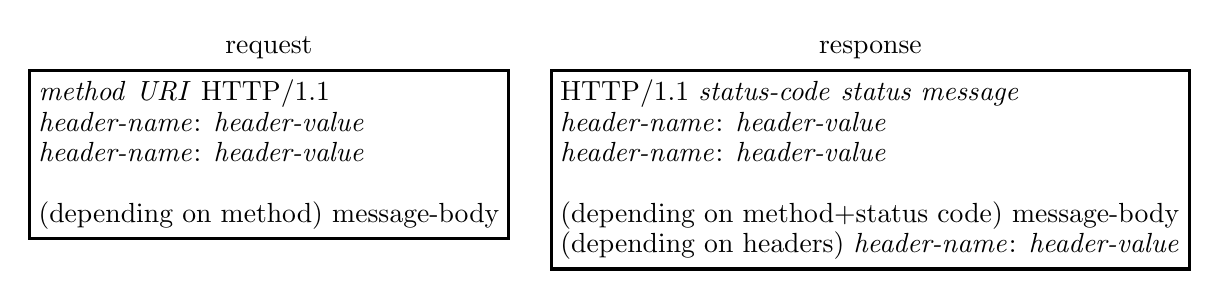
\begin{tikzpicture}
\node[draw,align=left,very thick,font=\fontsize{10}{11}\selectfont,label={north:request}] (request) {
\textit{method} \textit{URI} HTTP/1.1\\
\textit{header-name}: \textit{header-value} \\
\textit{header-name}: \textit{header-value} \\
~ \\
(depending on method) message-body
};
\node[anchor=north west,draw,align=left,font=\fontsize{10}{11}\selectfont,very thick,label={north:response}] 
at ([xshift=.5cm]request.north east){
HTTP/1.1 \textit{status-code} \textit{status message} \\
\textit{header-name}: \textit{header-value} \\
\textit{header-name}: \textit{header-value} \\
~ \\
(depending on method+status code) message-body \\
(depending on headers) \textit{header-name}: \textit{header-value}
};
\end{tikzpicture}
\end{frame}

\begin{frame}{HTTP/2, HTTP/3}
    \begin{itemize}
    \item `new' versions, not ubiquitously deployed
        \begin{itemize}
        \item HTTP/2: over TCP \textit{or} over TLS over TCP
        \item HTTP/3: over QUIC over UDP
        \end{itemize}
    \vspace{.5cm}
    \item multiple `streams' within one connection 
    \item send series of `frames' with stream ID + type + data
    \item frame types include:
        \begin{itemize}
        \item HEADERS --- encode message headers (key/value pairs)
        \item DATA --- include message bodies
        \end{itemize}
    \item method, status-code, URI encoded as special headers
    \end{itemize}
\end{frame}

\begin{frame}{HTTP/1.1 example (GET)}
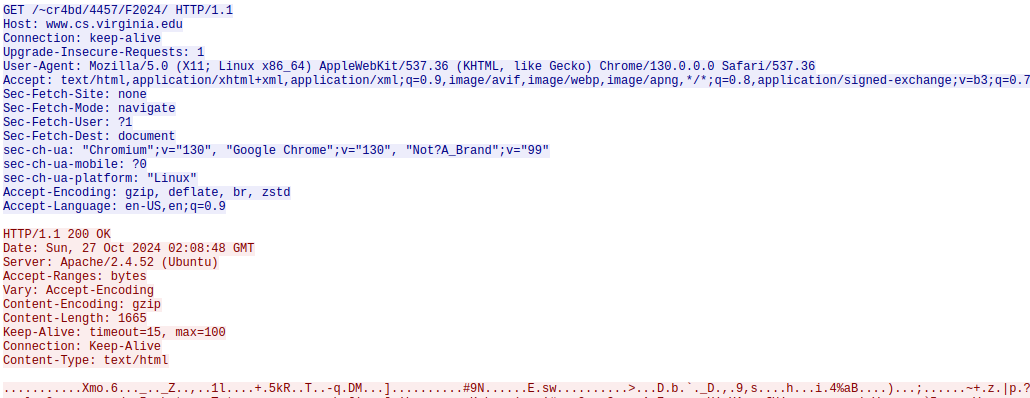
\includegraphics[width=\textwidth]{../http/http-wireshark-simple}
\end{frame}

\begin{frame}{HTTP/2.0 example (GET request)}
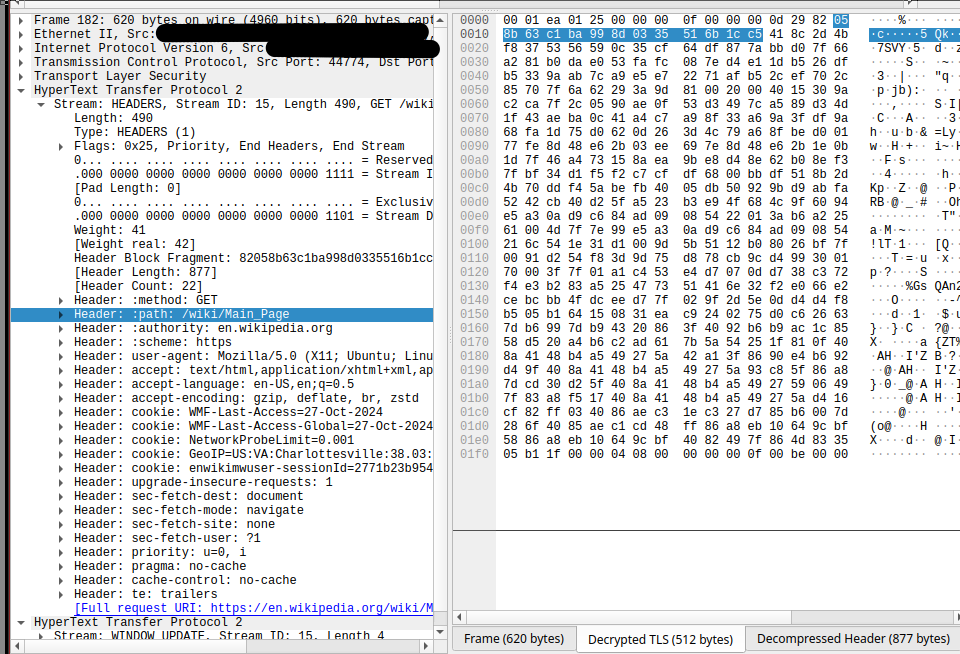
\includegraphics[width=\textwidth]{../http/http2-get-ex}
\end{frame}

% FIXME: HTTP/2.0 response

\begin{frame}{HTTP/1.1 example (POST)}
% FIXME
\end{frame}


\section{HTTP methods, briefly}
\begin{frame}{selected HTTP methods}
\small
\begin{tabular}{lllll}
method & purpose & request body? & respones body? & `safe' \\
GET & retrieve resource & never & usually & yes \\
HEAD & retrieve resource headers& never & never & yes \\
POST & provide data & always & usually & no \\
PUT & set contents of resource & always & maybe & no \\
DELETE & delete resource & never & maybe & no \\
OPTIONS & get info about server & maybe & maybe & no \\
\end{tabular}
\end{frame}

\begin{frame}{safety}
    \begin{itemize}
    \item GET, HEAD = `safe' methods
    \item okay for clients to repeat, send unprompted
        \begin{itemize}
        \item `prefetch' resources
        \item redo when user presses back button unprompted
        \end{itemize}
    \item other methods: that's not okay!
    \end{itemize}
\begin{center}
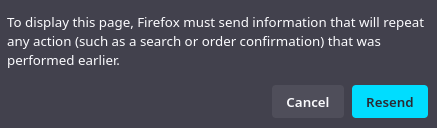
\includegraphics[width=0.7\textwidth]{../http/ff-resend-warning}
\end{center}
\end{frame}



\section{HTTP POST}
\begin{frame}[fragile]{HTTP POST}
\begin{Verbatim}[fontsize=\small]
POST /cs4457-fall2024-quiz-listener.php HTTP/1.1
Host: kytos02-noauth.cs.virginia.edu
Content-Type: application/json
Content-Length: 184
...

{"user":"cr4bd","realuser":"cr4bd","session_id":"abcdefabcdef0123456789aaaaaaaaaaaaaaaaaaaaaaaaaaaaaaaaaaaaaaaaaa","quiz":"week09","slug":"71d45222","answer":["d2f4e81b"],"sequence":0}
\end{Verbatim}
\end{frame}

\begin{frame}[fragile]{HTML forms (GET)}
\begin{tikzpicture}
\node[align=left,font=\fontsize{8}{9}\selectfont] (html) {
\begin{minipage}{0.6\textwidth}
\begin{Verbatim}
<form action="https://example.com/foo" method="get">
Name: <input type="text" name="name"><br>
Query: <input type="text" name="query"><br>
<input type="submit" value="Submit">
</form>
\end{Verbatim}
\end{minipage}
};
\node[anchor=north east] (pic) at (html.north west) {
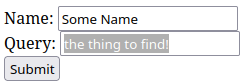
\includegraphics[width=0.3\textwidth]{../http/html-form-get.png}
};
\end{tikzpicture}
\begin{Verbatim}[fontsize=\small]
GET /foo?name=Some+Name&query=the+thing+to+find%21 HTTP/1.1
Host: example.com
...
\end{Verbatim}
\end{frame}

\begin{frame}[fragile]{HTML forms (POST)}
\begin{tikzpicture}
\node[align=left,font=\fontsize{8}{9}\selectfont] (html) {
\begin{minipage}{0.6\textwidth}
\begin{Verbatim}
<form action="https://example.com/foo" method="post">
Name: <input type="text" name="name"><br>
Comment:
<textarea name="comment">
</textarea>
<br>
<input type="submit" value="Submit">
</form>
\end{Verbatim}
\end{minipage}
};
\node[anchor=north east] (pic) at (html.north west) {
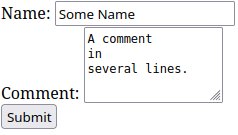
\includegraphics[width=0.3\textwidth]{../http/html-form-post.png}
};
\end{tikzpicture}
\begin{Verbatim}[fontsize=\small]
POST /foo HTTP/1.1
Host: example.com
Content-Type: application/x-www-form-urlencoded
Content-Length: 60
...

name=Some+Name&comment=A+comment%0D%0Ain%0D%0Aseveral+lines.
\end{Verbatim}
\end{frame}

\begin{frame}[fragile]{HTML forms (multipart/form-data)}
\begin{Verbatim}[fontsize=\fontsize{9}{10}]
<form action="https://example.com/foo" method="post"
    enctype="multipart/form-data">
    ...
\end{Verbatim}
\rule{0.9\textwidth}{1mm}
\begin{Verbatim}[fontsize=\fontsize{9}{10}]
POST /foo HTTP/1.1
Host: example.com
Content-Type: multipart/form-data; boundary=---------------------------81545828010202052201987031310
Content-Length: 321
...

-----------------------------30871118663472832060210928793
Content-Disposition: form-data; name="name"

Some Name
-----------------------------30871118663472832060210928793
Content-Disposition: form-data; name="comment"

A comment
in
several lines.
-----------------------------30871118663472832060210928793--
\end{Verbatim}
\end{frame}

\begin{frame}{GET v POST}
\begin{tabular}{p{7cm}|p{7cm}}
GET & POST \\ \hline
works with back button, caches & not resent automatically \\
limited by URL size & huge possible size \\
saving URL accesses page again & form info never `leaked' in browser history, referer, etc.\\
only simple text fields & supports file uploads (via multipart/form-data) \\
\end{tabular}
\end{frame}



\section{exercise: HTTP which}
\begin{frame}{exercise: which method}
    \begin{itemize}
    \item GET or POST or something else for
    \vspace{.5cm}
    \item image that shows a clock with current time
    \item rating a product and displaying the resulting summary of all ratings
    \item search query for a Twitter-like website
    \item getting the 2nd page of search results
    \end{itemize}
\end{frame}


\section{virtual hosting, Host header}
\begin{frame}[fragile]{multiple names, one IP}
\begin{Verbatim}
$ dig +short es.wikipedia.org aaaa
dyna.wikimedia.org.
2620:0:860:ed1a::1
$ dig +short en.wikipedia.org aaaa
dyna.wikimedia.org.
2620:0:860:ed1a::1
\end{Verbatim}
\begin{itemize}
\item how does this work?
\end{itemize}
\end{frame}

\begin{frame}{Host/:authority header}
\begin{itemize}
\item when getting http://somehostname/path, send header
\item \texttt{Host: somehostname} (HTTP/1.1)
\item \texttt{:authority: somehostname} (HTTP/2, HTTP/3)
\vspace{.5cm}
\item allows for `virtual hosts'
\end{itemize}
\end{frame}


\section{error codes}
\begin{frame}{selected HTTP status codes}
\begin{itemize}
\item 1xx --- informational
\item 2xx --- successful
    \begin{itemize}
    \item 200 OK, 204 No Content
    \end{itemize}
\item 3xx --- redirection
    \begin{itemize}
    \item 301 Moved Permanently, 302 Found, 303 See Other
    \item `Location' header gives next URL to use
    \item 304 Not Modified (conditional GET --- later)
    \end{itemize}
\item 4xx --- client error
    \begin{itemize}
    \item 403 Forbidden, 404 Not Found
    \end{itemize}
\item 5xx --- server error
\end{itemize}
\end{frame}

% FIXME

\section{persistent, pipelining}
% FIXME: pipelining screenshot
\begin{frame}{one connection, multiple requests}
    \begin{itemize}
    \item HTTP/0.9, HTTP/1.0 --- one request+response per connection
        \begin{itemize}
        \item big efficiency problem
        \end{itemize}
    \item solution 1: persistent connections
    \item solution 2: pipelining
    \item solution 3 (HTTP/2+): multiple `streams' in one connection
    \end{itemize}
\end{frame}

\begin{frame}{end-of-request/response}
    \begin{itemize}
    \item body of request/response can be variable length
    \vspace{.5cm}
    \item so when does request/response end if it has a body?
    \item HTTP/1.0 original solution (RFC 1945)
        \begin{itemize}
        \item ``the length of that body may be determined in two ways. If a Content-Length field is present, the value in bytes represents the length of the Entity-Body. Otherwise, the body length is determined by the closing of the connection by the server.''
        \end{itemize}
    \item advantage of latter idea: don't need to generate whole document before sending headers
    \item disadvantage: no persistent connections!
    \end{itemize}
\end{frame}


\providecommand{\chunksize}[1]{\textbf{\color{violet!80}#1}}
\begin{frame}[fragile,label=chunked]{chunked transfer coding}
\begin{Verbatim}[commandchars=\\\{\}]
HTTP/1.1 200 OK
Content-Type: text/plain
\textbf{Transfer-Coding: chunked}
...

\chunksize{1B}
\textbf{This is 0x1B bytes of text.}
\chunksize{21}
\textbf{And 0x21 bytes}
\textbf{with more lines.}
\chunksize{0}
\end{Verbatim}
\end{frame}

\begin{frame}{pipelining}
\begin{tikzpicture}
\tikzset{
    nodeline/.style={draw,ultra thick},
    msgline/.style={draw,very thick,-Latex},
    msgbox/.style={draw,fill=white,font=\small\tt,align=left},
}
\draw[nodeline] (0, -.5) -- ++(0, -7) node[pos=0,above] {client};
\draw[nodeline] (12, -.5) -- ++(0, -7) node[pos=0,above] {server};
\draw[msgline] (0, -1) -- (12, -2) node[midway,msgbox] {
    GET /image1.png HTTP/1.1
    \ldots
};
\draw[msgline] (0, -1.5) -- (12, -2.5) node[midway,msgbox] {
    GET /image2.png HTTP/1.1
    \ldots
};
\draw[msgline] (0, -2) -- (12, -3) node[midway,msgbox] {
    GET /script.js HTTP/1.1
    \ldots
};
\draw[msgline] (12, -2.5) -- (0, -3) node[midway,below,msgbox] {
    HTTP/1.1 200 OK
    \ldots
};
\draw[msgline] (12, -4) -- (0, -5) node[midway,msgbox] {
    HTTP/1.1 200 OK
    \ldots
};
\draw[msgline] (12, -5) -- (0, -6) node[midway,msgbox] {
    HTTP/1.1 200 OK
    \ldots
};
\end{tikzpicture}
\end{frame}

\begin{frame}{HTTP/1.1 `pipelining'}
    \begin{itemize}
    \item send series of requests before receiving any response
    \item potentailly server can potentially process requests in parallel
    \vspace{.5cm}
    \item need to handle resending requests if connection dropped early
    \end{itemize}
\end{frame}

\begin{frame}{HTTP/2.0 multiple streams}
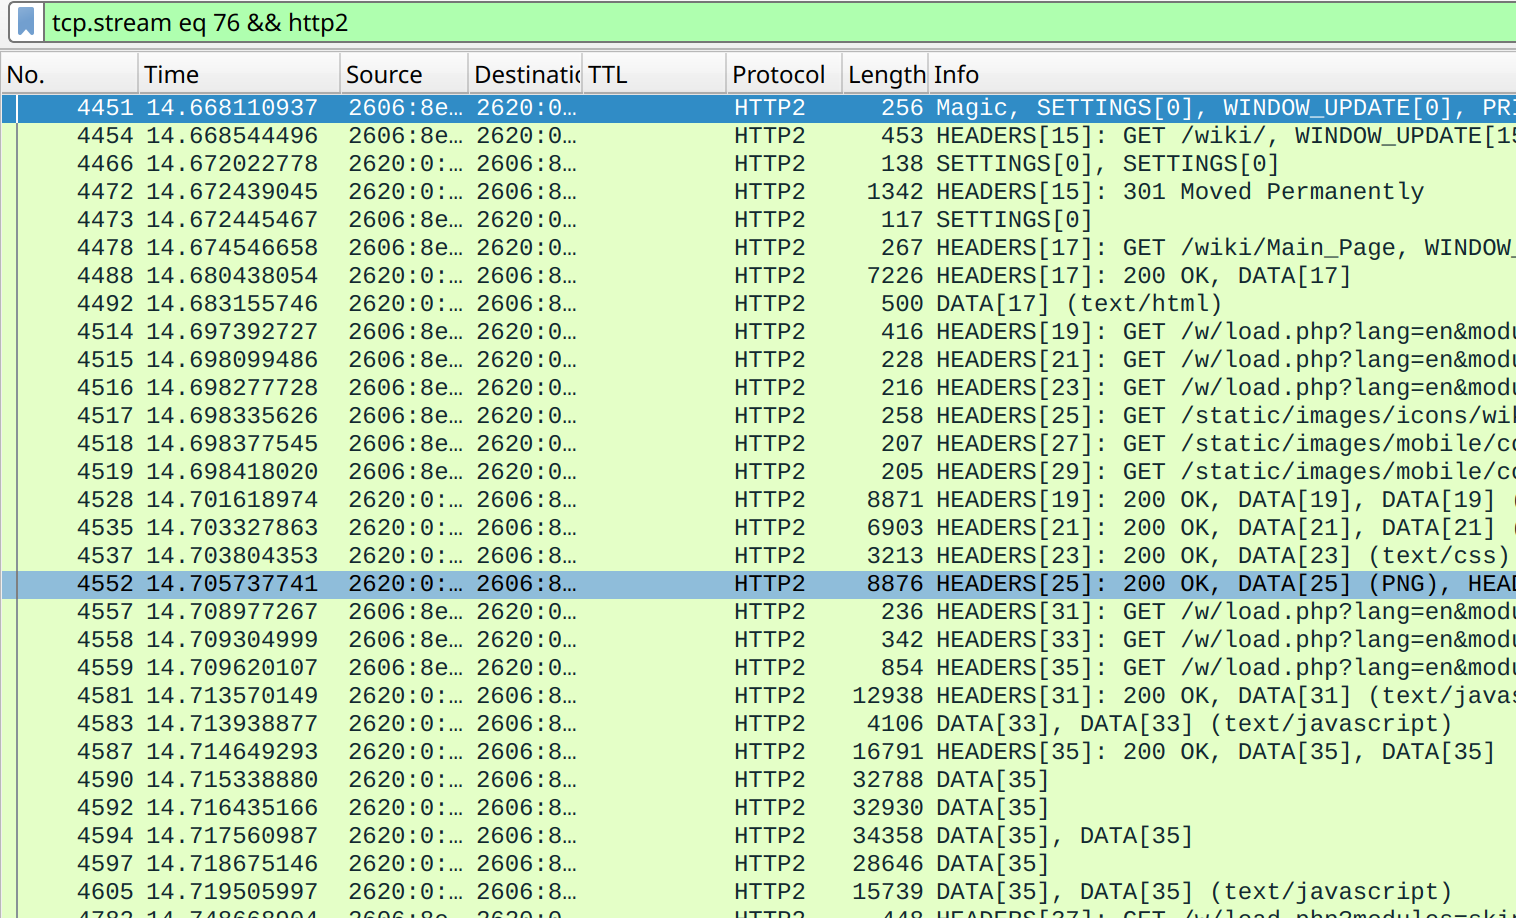
\includegraphics[width=\textwidth]{../http/http2-multi-reqres}
\end{frame}


\section{content negotiation}
\begin{frame}{content negotiation}
\begin{itemize}
\item Firefox on my desktop $\rightarrow$ wikipedia:
\item {\small\texttt{accept: text/html,application/xhtml+xml,application/xml;q=0.9,image/avif,image/webp,image/png,image/svg+xml,*/*;q=0.8}}
    \begin{itemize}
    \item list of formats and preference indicator for each (\texttt{q})
    \item described using ``media types'' (RFC 6838)
    \end{itemize}
\item {\small\texttt{accept-language: en-US,en;q=0.5}}
\item {\small\texttt{accept-encoding: gzip, deflate, br, zstd}}
    \begin{itemize}
    \item allowed compression formats
    \end{itemize}
\end{itemize}
\end{frame}

\begin{frame}{advice against content negotation}
\begin{itemize}
\item current HTTP standard (RFC 9110) says this approach ``has several disadvantages'':
    \begin{itemize}
    \item advises considering approaches where client chooses version
    \end{itemize}
\item `impossible for the server to accurately determine what might be ``best'' '
\item `having the [client] describe its capabilities in every request can be very inefficient \ldots and a potential risk to the user's privacy'
\item `complicates the implementation'
\item `limits \ldots shared caching'
\end{itemize}
\end{frame}


\section{cookies}
\begin{frame}{HTTP non-state}
    \begin{itemize}
    \item HTTP is a `stateless'
    \item each request stands on its own
        \begin{itemize}
        \item processed independently of all other requests
        \item even if multiple in a connection
        \end{itemize}
    \vspace{.5cm}
    \item this is disappointing for websites: \\
    supporting `login' functionality \\
    supporting user preferences
    \end{itemize}
\end{frame}

\begin{frame}[fragile]{HTTP cookies (RFC 6265)}
example.com $\rightarrow$ client
\begin{Verbatim}[fontsize=\small]
HTTP/1.1 200 OK
Set-Cookie: SessionID=31d4d96e407aad42; Path=/; Domain=example.com
\end{Verbatim}
client $\rightarrow$ example.com on later requests:
\begin{Verbatim}[fontsize=\small]
GET /some-path HTTP/1.1
Host: example.com
Cookie: SessionID=31d4d96e407aad42
\end{Verbatim}
\end{frame}


\begin{frame}{session ID concept}
    \begin{itemize}
    \item assign random ID number to each `session' if no cookie set
    \vspace{.5cm}
    \item in some database:
    \item if they add to shopping cart, associate ID number with shopping cart items
    \item if user logs in, associate ID number with user
    \item \ldots
    \end{itemize}
\end{frame}

\begin{frame}{selected cookie attributes}
\begin{itemize}
\item domain --- limit to subset of domains
    \begin{itemize}
    \item domain=example.com matches example.com, foo.example.com, but not other.com
    \end{itemize}
\item secure --- only send back on encrypted connections
\item httponly --- do not expose to in-webpage scripts
\item expires, max-age --- limit how long cookie kept around
    \begin{itemize}
    \item default = until browser closed
    \end{itemize}
\end{itemize}
\end{frame}

\begin{frame}{cookies and tracking}
    \begin{itemize}
    \item cookies often used for tracking users \textit{across websites}
    \item and not by setting cookies valid for tons of domains
    \vspace{.5cm}
    \item how: websites load data from other websites
        \begin{itemize}
        \item separate HTTP requests with separate cookies
        \end{itemize}
    \end{itemize}
\end{frame}

\begin{frame}{cookie tracking example}
\begin{itemize}
\item foo.com, bar.com, quux.com all include an image
    \begin{itemize}
    \item https://tracker.com/track-XXX.png where XXX is foo, bar or quux
    \end{itemize}
\item tracker.com can read cookie every time image is accessed
    \begin{itemize}
    \item and set a cookie to unique number if not set
    \end{itemize}
\item now tracker.com knows:
    \begin{itemize}
    \item when/if every visitor of foo.com visited bar.com and/or quux.com
    \end{itemize}
\end{itemize}
\end{frame}

\begin{frame}{more detailed tracking?}
    \begin{itemize}
    \item ``just'' learned about how many visitors visited combinations of websites
    \item with some cooperation can get more info:
        \begin{itemize}
        \item which subpages on those websites
        \item username or email entered into those websites
        \item \ldots
        \end{itemize}
    \item one way to pass info: add extra data to image filename
    \end{itemize}
\end{frame}

\begin{frame}{third party cookie rules}
    \begin{itemize}
    \item some browsers might restrict `third-party cookies'
        \begin{itemize}
        \item cookies sent to Y because of visit to X
        \end{itemize}
    \item various options, with variable deployment:
        \begin{itemize}
        \item only make third-party cookies work if marked SameSite=None
        \item separate cookie storage for each `root' website
        \item ignore cookies from unvisited sites
        \item disable only cookies that heuristically look like tracking
        \end{itemize}
    \end{itemize}
\end{frame}


\section{caching}
\begin{frame}{HTTP caching (RFC 9111)}
    \begin{itemize}
    \item making webpages fast --- let clients cache values for later
    \item some problems:
    \vspace{.5cm}
    \item how to tell if something's out of date
    \item how to tell if changes to cookies/accept-language/etc. change item
    \end{itemize}
\end{frame}

\begin{frame}<1>[label=oodOpt]{is it out of date? options}
    \begin{itemize}
    \item \myemph<2>{expire date; max-age in seconds}
    \item \myemph<3>{check with server if it has changed}
    \end{itemize}
\end{frame}

\againframe<2>{oodOpt}

\begin{frame}[fragile]{expires}
\begin{Verbatim}
HTTP/1.1 200 OK
Date: Mon, 28 Oct 2024 00:29:02 GMT
Expires: Mon, 28 Oct 2024 04:29:02 GMT
...
\end{Verbatim}
\rule{0.9\textwidth}{1mm}
\begin{Verbatim}
HTTP/1.1 200 OK
Cache-Control: max-age=14400
...
\end{Verbatim}
\end{frame}

\againframe<3>{oodOpt}

\begin{frame}[fragile]{conditional GETs}
\begin{Verbatim}[fontsize=\fontsize{12}{13}]
GET /3/library/struct.html HTTP/1.1
...

HTTP/1.1 200 OK
Date: Sun, 27 Oct 2024 20:01:15 GMT
Last-Modified: Sun, 27 Oct 2024 18:50:46 GMT
ETag: "671e8b86-13e32"
\end{Verbatim}
\rule{0.9\textwidth}{1mm}
\begin{Verbatim}[fontsize=\fontsize{12}{13}]
GET /3/library/struct.html HTTP/1.1
If-Modified-Since: Sun, 27 Oct 2024 18:50:46 GMT
If-None-Match: "671e8b86-13e32"
...
HTTP/1.1 304 Not Modified
...
\end{Verbatim}
\end{frame}

\begin{frame}[fragile]{variable responses}
\begin{Verbatim}
HTTP/1.1 200 OK
...
Vary: Accept, Accept-Lnaguage, Cookie
...
\end{Verbatim}
\begin{itemize}
\item page contents may vary even though URL doesn't change
\item Vary header says what things need to be the same
\item typically used to discard cached responses
\end{itemize}
\end{frame}

\begin{frame}[fragile]{other cache-control settings}
\begin{itemize}
\item seen max-age=X, also\ldots
\item no-store
    \begin{itemize}
    \item do not store a copy of this response
    \end{itemize}
\item no-cache
    \begin{itemize}
    \item do not use without checking for new version first (conditional GET or similar)
    \end{itemize}
\item private, public
    \begin{itemize}
    \item indicate if acceptable for cache shared between users
    \end{itemize}
\end{itemize}
\end{frame}


\section{proxies and reverse proxies}
\usetikzlibrary{arrows.meta}
\begin{frame}{HTTP proxies (1)}
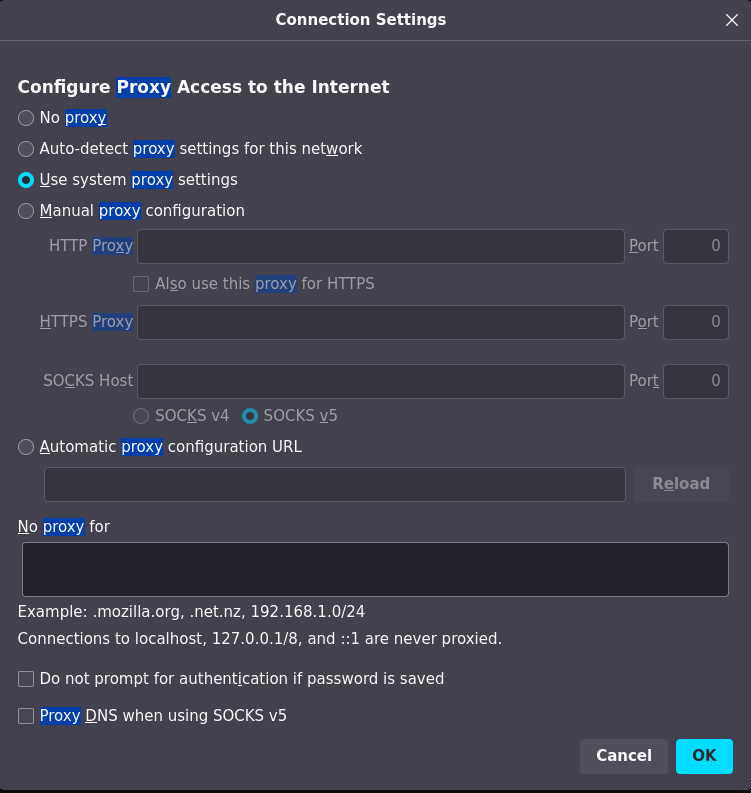
\includegraphics[height=0.9\textheight]{../http/moz-proxy-config}
\end{frame}

\begin{frame}
\begin{tikzpicture}
\node[draw, very thick,align=center] (user agent) at (0, 0) {
    user-agent \\ (example: \\ web browser)
};
\node[draw, very thick,align=center] (proxy) at (6, 0) {
    proxy \\server
};
\node[draw, very thick,align=center] (web server) at (12, 0) {
    web \\server
};
\draw[thick,Latex-Latex] (user agent) -- (proxy)
    node[pos=0,above right] {client}
    node[pos=1,above left] {server}
    coordinate[midway] (midpt cp);
\draw[thick,Latex-Latex] (proxy) -- (web server)
    node[pos=0,above right] {client}
    node[pos=1,above left] {server}
    coordinate[midway] (midpt ps);
\draw (midpt cp) -- ++(0cm, -1cm) node[below,align=center] {
    request specifies \\
    which web server \\
    to contact
};
\draw (midpt ps) -- ++(0cm, -1cm) node[below,align=center] {
    looks like normal \\
    user-agent request 
};
\end{tikzpicture}
\end{frame}

\begin{frame}[fragile]{HTTP proxies (2)}
browser$\rightarrow$HTTP(S) proxy sever: \\
\begin{Verbatim}
GET http://example.com/somesite HTTP/1.1
Host: example.com
...
\end{Verbatim}
\rule{.9\textwidth}{1mm}
\begin{itemize}
    \item instead of path, can put full URL
    \item doesn't have to be \texttt{http} URL
\end{itemize}
\end{frame}

\begin{frame}{proxy functionality}
    \begin{itemize}
    \item caching for multiple users
        \begin{itemize}
        \item reason for \texttt{Cache-Control: private}
        \end{itemize}
    \item filtering content
        \begin{itemize}
        \item antimalware, adblocking, etc.
        \end{itemize}
    \item logging content (example: debugging webapp)
    \item \ldots
    \end{itemize}
\end{frame}

\begin{frame}
\begin{tikzpicture}
\node[draw, very thick,align=center] (user agent) at (0, 0) {
    user-agent \\ (example: \\ web browser)
};
\node[draw, very thick,align=center] (proxy) at (6, 0) {
    forward proxy \\server
};
\node[draw, very thick,align=center] (web server) at (12, 0) {
    web \\server
};
\draw[thick,Latex-Latex] (user agent) -- (proxy)
    node[pos=0,above right] {client}
    node[pos=1,above left] {server}
    coordinate[midway] (midpt cp);
\draw[thick,Latex-Latex] (proxy) -- (web server)
    node[pos=0,above right] {client}
    node[pos=1,above left] {server}
    coordinate[midway] (midpt ps);
\draw (midpt cp) -- ++(0cm, -1cm) node[below,align=center] {
    request specifies \\
    which web server \\
    to contact
};
\draw (midpt ps) -- ++(0cm, -1cm) node[below,align=center] {
    looks like normal \\
    user-agent request 
};

\begin{scope}[yshift=-5cm,name prefix=rvs-]
\node[draw, very thick,align=center] (user agent) at (0, 0) {
    user-agent \\ (example: \\ web browser)
};
\node[draw, very thick,align=center] (proxy) at (6, 0) {
    reverse proxy \\server
};
\node[draw, very thick,align=center] (web server) at (12, 0) {
    backend\\server
};
\draw[thick,Latex-Latex] (user agent) -- (proxy)
    node[pos=0,above right] {client}
    node[pos=1,above left] {server}
    coordinate[midway] (midpt cp);
\draw[thick,Latex-Latex] (proxy) -- (web server)
    node[pos=0,above right] {client}
    node[pos=1,above left] {server}
    coordinate[midway] (midpt ps);
\draw (midpt cp) -- ++(0cm, -1cm) node[below,align=center] {
    looks like normal \\
    user-agent request
};
\draw (web server) -- ++(-1cm, -1cm) node[below,align=center] {
    selected from \\
    user-agent request path
};
\end{scope}
\end{tikzpicture}
\end{frame}

\begin{frame}{reverse proxy}
    \begin{itemize}
    \item why not just go directly to actual web server?
    \vspace{.5cm}
    \item make multiple web severs appear as one? example:
        \begin{itemize}
        \item https://example.com/foo/XXX goes to https://foo-backend.example.com/XXX
        \item https://example.com/bar/XXX goes to https://bar-backend.example.com/XXX
        \item https://example.com/ goes to https://frontpage.example.com/
        \end{itemize}
    \item do caching, filtering, or similar on behalf of webservers
    \item split requests between multiple identical servers for performance
    \end{itemize}
\end{frame}


\subsection{aside: wikimedia architecture}
\begin{frame}{Wikimedia architecture}
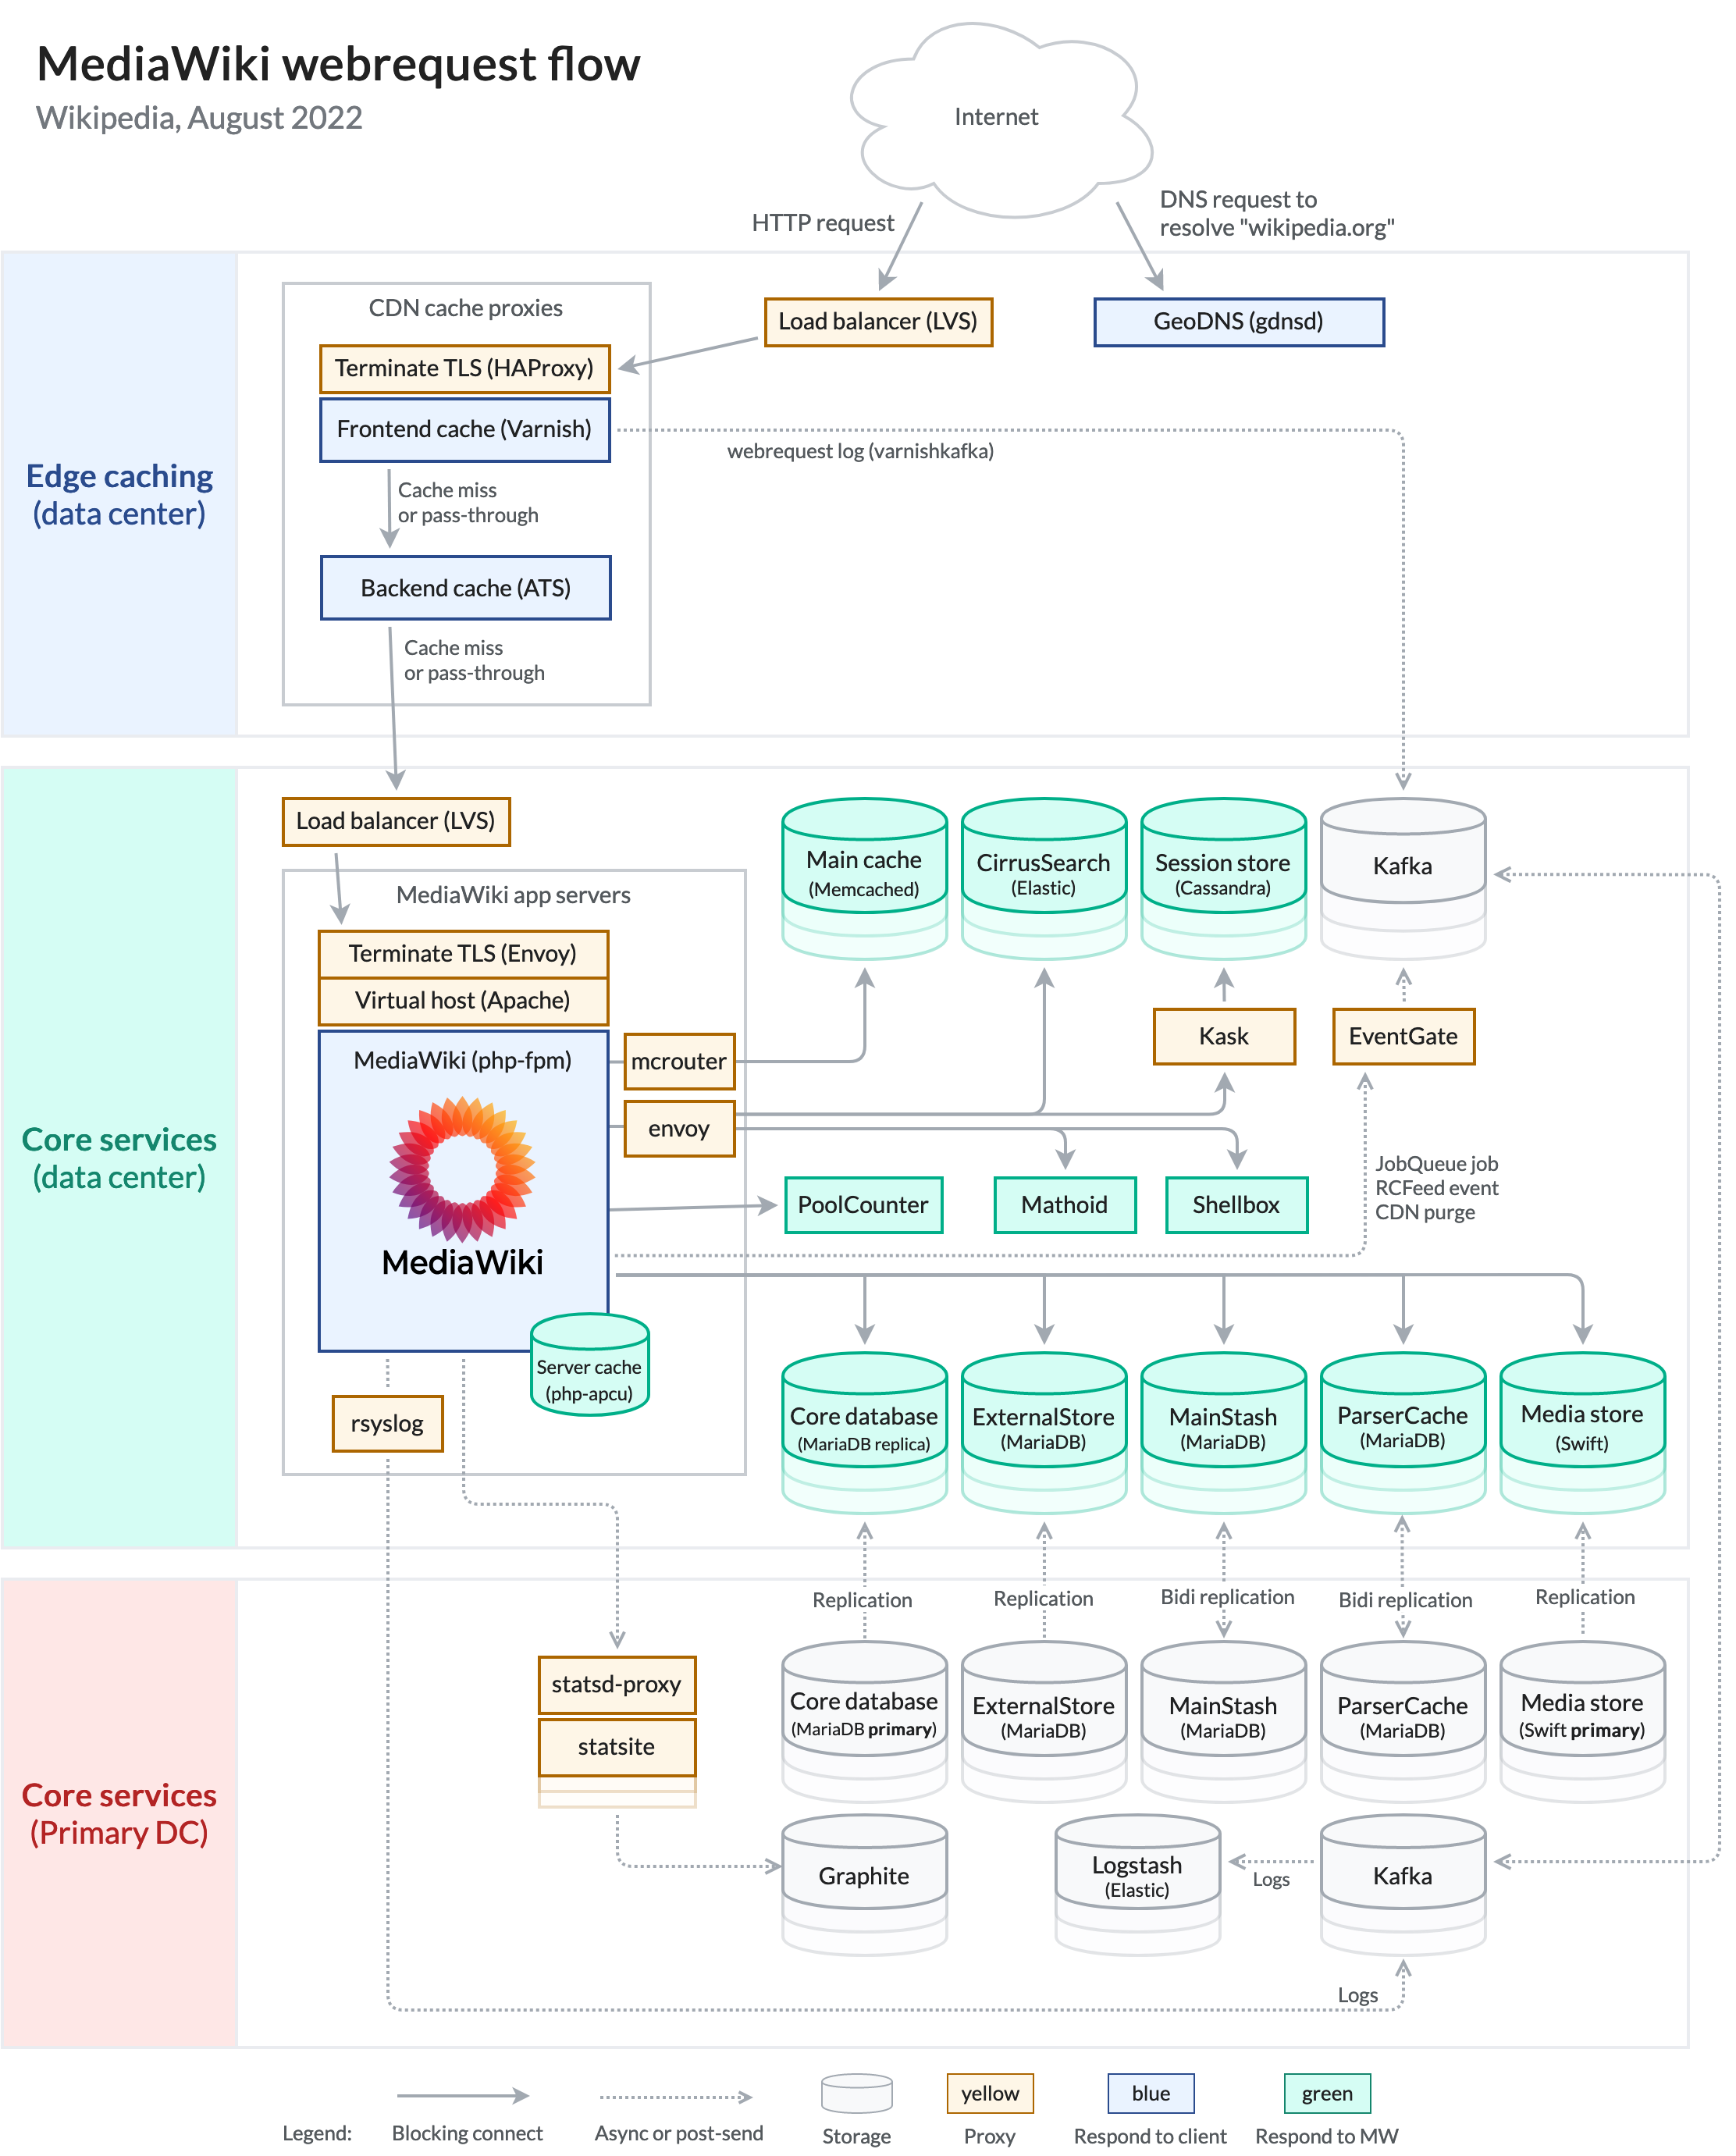
\includegraphics[height=0.85\textheight]{../http/Wikipedia_webrequest_2022.png}
\end{frame}


\section{REST}
\begin{frame}{REST}
    \begin{itemize}
    \item REpresentational State Transfer
    \item idea for application interface on top of HTTP
    \vspace{.5cm}
    \item entities in system represented with URLs
    \item GET requests to get state of that entity
    \item PUT and/or POST requests to update entity state
    \item DELETE requests to remove entity
    \end{itemize}
\end{frame}

\begin{frame}[fragile]{example: Canvas API for announcements (1)}
client $\rightarrow$ canvas HTTP server:
\begin{Verbatim}[fontsize=\fontsize{9}{10}\selectfont]
GET /api/v1/courses/123456/discussion_topics?only_announcements=true
Authorization: Bearer [secret code]
\end{Verbatim}
\rule{0.9\textwidth}{1mm}
\begin{Verbatim}[fontsize=\fontsize{9}{10}\selectfont]
HTTP/1.1 200 OK
...

[{
    "id":1,
    "title":"Welcome to the Course!",
    "message":"...",
    ...
},
{
    "id":2,
    ...
\end{Verbatim}
\end{frame}

\begin{frame}[fragile]{example: Canvas API for announcements (2)}
client $\rightarrow$ canvas HTTP server:
\begin{Verbatim}[fontsize=\fontsize{9}{10}\selectfont]
POST /api/v1/courses/123456/discussion_topics
Authorization: Bearer [secret code]
Content-Type: application/json
...

{
    "is_announcement":true,
    "title":"Class Cancelled",
    "message":"....."
}
\end{Verbatim}
\rule{0.9\textwidth}{1mm}
\begin{Verbatim}[fontsize=\fontsize{9}{10}\selectfont]
HTTP/1.1 200 OK
...

{
    "id": 41,
    "title":"Class Cancelled",
    ....
}
\end{Verbatim}
\end{frame}

\begin{frame}[fragile]{example: Canvas API for announcements (3)}
client $\rightarrow$ canvas HTTP server:
\begin{Verbatim}[fontsize=\fontsize{9}{10}\selectfont]
PUT /api/v1/courses/123456/discussion_topics/41
Authorization: Bearer [secret code]
Content-Type: application/json
...

{
    "is_announcement":true,
    "title":"Class Cancelled [updated!]",
    "message":"UPDATE: prevoiusly,.."
    ...
}
\end{Verbatim}
\rule{0.9\textwidth}{1mm}
\begin{Verbatim}[fontsize=\fontsize{9}{10}\selectfont]
HTTP/1.1 200 OK
...

{
    "id": 41,
    "title":"Class Cancelled [updated!]",
    ....
}
\end{Verbatim}
\end{frame}



% FIXME: SOAP? HLS?


\section{backup slides}
\begin{frame}\frametitle{backup slides}
\end{frame}
\section{common record types}
\begin{frame}{selected RR types}
\begin{tabular}{l|l|l|p{6cm}}
text & id & purpose & data format \\ \hline
\texttt{A} & 1 & IPv4 address & 32-bit integer (big-endian) \\
\texttt{AAAA} & 28 & IPv6 address & 128-bit integer (big-endian) \\
\texttt{NS} & 2 & authoritative name server & domain name \\
\texttt{CNAME} & 5 & `canonical name' & domain name \\
\texttt{TXT} & 16 & text string & arbitrary string \\
\texttt{SRV} & 33 & service location & priority, weight, domain name, port \\
\end{tabular}
\end{frame}

\begin{frame}[fragile]{CNAME}
\begin{itemize}
\item CNAME = delegate name to another name
\end{itemize}
\begin{Verbatim}[fontsize=\small]
canvas.its.virginia.edu. 2711   IN      CNAME   \
    universityofvirginia-vanity.instructure.com.
universityofvirginia-vanity.instructure.com. 238 IN CNAME \
    canvas-pdx-prod-c354-1908777142.us-west-2.elb.amazonaws.com.
canvas-pdx-prod-c354-1908777142.us-west-2.elb.amazonaws.com. 2 IN A 34.208.211.157
canvas-pdx-prod-c354-1908777142.us-west-2.elb.amazonaws.com. 2 IN A 44.238.73.244
canvas-pdx-prod-c354-1908777142.us-west-2.elb.amazonaws.com. 2 IN A 52.26.9.245
\end{Verbatim}
\begin{itemize}
\item connecting to canvas.its.virginia.edu?
\item use one of 34.208.211.157, 44.238.73.244, 52.26.9.245
\end{itemize}
\end{frame}

\begin{frame}[fragile]{NS}
\begin{Verbatim}[fontsize=\small]
virginia.edu. 3600    IN      NS      uvaarpa.virginia.edu.
virginia.edu. 3600    IN      NS      nom.virginia.edu.
virginia.edu. 3600    IN      NS      eip-01-aws.net.virginia.edu.
\end{Verbatim}
\begin{itemize}
\item these three servers are authoritative for virginia.edu
\item (but need their A or AAAA records to actually contact them)
\end{itemize}
\end{frame}

\begin{frame}[fragile]{SRV}
\begin{Verbatim}
_ldap._tcp.virginia.edu. 600    IN      SRV     0 100 389 vadcv4.virginia.edu.
_ldap._tcp.virginia.edu. 600    IN      SRV     0 100 389 vadc5.virginia.edu.
\end{Verbatim}
\begin{itemize}
\item virginia.edu's LDAP servers are vadcv4.virginia.edu port 389 and vadc5.virginia.edu port 389
\item (LDAP = Lightweight Directory Access Protocol)
    \begin{itemize}
    \item example: lookup email ID by name
    \end{itemize}
\end{itemize}
\end{frame}

\begin{frame}{SRV records were late\ldots}
\begin{itemize}
\item SRV records seem like something we'd use all the time\ldots
\item but only used with a few protocols
\item why?
\vspace{.5cm}
\item SRV records added late (1996--2000)
\item sending email already had its own record type (MX)
\item poor support for querying them in standard networking libraries
\item hard to get access to add them in many organizations
\end{itemize}
\end{frame}

\begin{frame}[fragile]{dig virginia.edu txt}
\begin{Verbatim}[fontsize=\fontsize{8}{9}]
virginia.edu.           3548    IN      TXT     "google-site-verification=zEwuk4FIG8_vtv2BZJOD6IWzg9JbNiJPH9mQdPNCXRw"
virginia.edu.           3548    IN      TXT     "cisco-ci-domain-verification=268b991de3589451b38fcfeaa99473f8e4fb2522f96a1b478e04ec1bd5a25ff9"
virginia.edu.           3548    IN      TXT     "miro-verification=9f3238c881466b3ccb99c4347b99e5504eafc118"
virginia.edu.           3548    IN      TXT     "MS=ms40126609"
virginia.edu.           3548    IN      TXT     "onetrust-domain-verification=d901adf09116474c89790a9752e0046c"
virginia.edu.           3548    IN      TXT     "google-site-verification=rePHmrM7FEfSw62DHq9TpuMFUw66J6hgpFFh5cq89IM"
virginia.edu.           3548    IN      TXT     "v=spf1 a mx ip4:52.254.56.82 ip4:52.137.91.139 ip4:128.143.125.90 ip4:128.143.125.91 include:spf.protection.outlook.com include:_spf.google.com include:spf.elluciancloud.com ~all"
virginia.edu.           3548    IN      TXT     "docusign=6547d080-1c40-427c-8736-fafa466ff73f"
virginia.edu.           3548    IN      TXT     "apple-domain-verification=zllSamqSFAw4lNQo"
virginia.edu.           3548    IN      TXT     "v=msv1 t=537499f256ea46bd386f7543d18d28"
virginia.edu.           3548    IN      TXT     "atlassian-domain-verification=zeQ45p2Vl1fXekKYCzmq4ONEpDEkGKx3Y8Qzqe/8YV2ibzq6DLImIdTNw9Cv4lda"
virginia.edu.           3548    IN      TXT     "00256316"
virginia.edu.           3548    IN      TXT     "yYMwnn+VY4w6aVf+cE4888ppz+MDXBKnaI0m5eteiMGgwWIBTOgA6aTSJM4QYRG6s49MnR2Fj0grzaOKokmCow=="
virginia.edu.           3548    IN      TXT     "apple-domain-verification=mROwKUEMfwLBfltC"
virginia.edu.           3548    IN      TXT     "e2ma-verification=rx8eb"
virginia.edu.           3548    IN      TXT     "ZOOM_verify_PuU-eQzyQ7ONrij_vTP72A"
virginia.edu.           3548    IN      TXT     "sending_domain1023271=f4a69653389ff4543a64e982f1cbc2e9db30eab95cccfb8be58d883ce7849448"
\end{Verbatim}
\end{frame}

\begin{frame}{TXT record usage}
\begin{itemize}
\item TXT records `just' hold arbitrary strings
\item lots of machine-based usage of TXT records
\item probably in part because it's too slow/hard to add new record types
\end{itemize}
\end{frame}

\begin{frame}[fragile]{TXT example: SPF}
\begin{Verbatim}[fontsize=\small]
virginia.edu. 3548    IN      TXT "v=spf1 a mx
    ip4:52.254.56.82 ip4:52.137.91.139
    ip4:128.143.125.90 ip4:128.143.125.91
    include:spf.protection.outlook.com
    include:_spf.google.com
    include:spf.elluciancloud.com ~all"
\end{Verbatim}
\begin{itemize}
\item SPF protocol for specifying who can send email from domain
\item why in TXT record instead of its own type?
\end{itemize}
\end{frame}

\begin{frame}{RFC 6686, Appendix A excerpt} 
\fontsize{13}{14}\selectfont
At the time of SPF's initial development, the prospect of getting an
RRTYPE allocated for SPF was not seriously considered, partly because
doing so had high barriers to entry\ldots.

\vspace{.5cm}

Later, after RRTYPE 99 was assigned \ldots
a plan was put into place to effect a gradual
transition to using RRTYPE 99 instead of using RRTYPE 16.
This plan failed to take effect for four primary reasons:\ldots

\vspace{.5cm}

1.\ldots existing nameservers (and, in fact, DNS-aware firewalls) would drop or
reject requests for unknown RRTYPEs \ldots

\vspace{.5cm}

2. many DNS provisioning tools \ldots
   were, and still are, typically lethargic about
   adding support for new RRTYPEs

\vspace{.5cm}

\ldots
\end{frame}


\end{document}
